\documentclass[xcolor=dvipsnames]{beamer}
%\documentclass[handout,xcolor=dvipsnames,pdftex,hyperref={colorlinks=false}]{beamer}
\usetheme[height=7mm]{Rochester}
\setbeamertemplate{items}[ball]
\setbeamertemplate{blocks}[rounded][shadow=true]
\usepackage{xcolor}
\usepackage{colortbl}
\usepackage{multirow}
\usepackage{amsmath}
\usepackage{amsfonts}
\usepackage{epsfig}
%\usepackage{rotating}
%\usepackage{theorem}
\usepackage{times}
\usepackage[T1]{fontenc}
\usepackage{inconsolata}
\usepackage{fancyvrb}
\usepackage{bbm}

% == theme & colors
\usetheme{Warsaw}  % Jens' previous
%\usepackage{helvet}
\definecolor{someblue}{rgb}{0,.1,0.8}

\title{PS200C: Regression Discontinuity Designs}
%\subtitle[ ]{Instrumental Variables: Modern Perspective with Heterogeneous Treatment Effects}
\author{Chad Hazlett}
\institute[UCLA]{UCLA\\[1ex]
  \texttt{chazlett@ucla.edu}}

\definecolor{dgreen}{rgb}{0,.6,0.8}
\newtheorem{assumption}{Assumption}
\newtheorem{iass}{Identification Assumption}
\newtheorem{ires}{Identification Result}
\newtheorem{estm}{Estimand}
\newtheorem{esti}{Estimator}
\newtheorem{question}{Question}
\newtheorem{answer}{Answer}
\newtheorem{proposition}{Proposition}
\newcommand{\bs}{\boldsymbol}
\newcommand{\mb}{\mathbf}
\newcommand{\real}{\mathbb{R}}
\renewcommand{\u}{\ensuremath{\mb{u}}}
\renewcommand{\v}{\ensuremath{\mb{v}}}
\newcommand{\U}{\ensuremath{\mb{U}}}
\newcommand{\Z}{\ensuremath{\mb{Z}}}
\newcommand{\PP}{\ensuremath{\mb{P}}}
\newcommand{\M}{\ensuremath{\mb{M}}}
\newcommand{\X}{\ensuremath{\mb{X}}}
\newcommand{\x}{\ensuremath{\mb{x}}}
\newcommand{\Y}{\ensuremath{\mb{Y}}}
\newcommand{\K}{\ensuremath{\mb{K}}}

\newcommand{\D}{\ensuremath{\mb{D}}}
\newcommand{\y}{\ensuremath{\mb{y}}}
\renewcommand{\b}{\ensuremath{\bs{\beta}}}
\newcommand{\e}{\ensuremath{\bs{\epsilon}}}
\newcommand{\bhat}{\ensuremath{\hat{\bs{\beta}}}}
\newcommand{\XX}{\ensuremath{\X'\X}}
\newcommand{\XXinv}{\ensuremath{\left(\XX\right)^{-1}}}
\newcommand{\hatsig}{\ensuremath{\hat{\sigma}^2}}
\newcommand{\sig}{\ensuremath{\sigma^2}}
\newcommand{\hatmat}{\ensuremath{\X \XXinv \X'}}
\newcommand{\ehat}{\ensuremath{\hat{\e}}}
\newcommand{\tr}{\text{tr}}
\newcommand{\Sig}{\ensuremath{\bs{\Sigma}}}
\newcommand{\SigInv}{\ensuremath{\bs{\Sigma^{-1}}}}
\newcommand{\W}{\ensuremath{\mb{W}}}
\newcommand\E{\mathbb{E}}

\newcommand{\indep}{{\bot\negthickspace\negthickspace\bot}}
\useoutertheme{infolines}
\begin{document}

%
%\AtBeginSubsection[]
%{
%  \begin{frame}<beamer>
%    \frametitle{Outline}
%    \tableofcontents[currentsection,currentsubsection]
%  \end{frame}
%}

\begin{frame}
  \titlepage
\end{frame}

\begin{frame}{Roadmap}
\begin{enumerate}
\item Theory: Potential outcomes, identification, key quantities
\item Randomization
\begin{itemize}
\item difference in means, variance estimation
\item covariate adjustment
\item blocking
\item cluster randomization
\end{itemize}
\item Selection on Observables
\begin{itemize}
\item sub-classification
\item matching (on $X$)
\item weighting (on $X$)
\item matching and weighting on $Pr(D=1)$ (propensity scores)
\item regression 
\item sensitivity
\end{itemize}
\item Difference in Differences 
\item Instrumental Variables
\item Regression Discontinuity: Sharp, Fuzzy
\end{enumerate}
\end{frame}

\begin{frame}
  \frametitle{Regression Discontinuity Design (RDD)}
  \begin{itemize}
    \item<1-> RDD is a fairly old idea (Thistlethwaite and Campbell, 1960) but this design experienced a renaissance in recent years. \bigskip
   \item<2-> Assignment to treatment and control is not random, but:
\begin{itemize}
\item<3-> there is a rule influencing how people are assigned
\item<4-> at some boundary, a trivial change in expected potential outcome corresponds to a big change in probability of treatment
\item<5-> effect estimated is hopefully dominated by effect with only small role for bias.
\end{itemize}
\bigskip
\item<6-> Widely applicable in a rule based world (administrative programs, elections, etc.)\bigskip
\item<7-> High internal validity, poor external validity
\end{itemize}
\end{frame}


\section{Sharp Regression Discontinuity Design}

\subsection{Identification}

\begin{frame}
  \frametitle{Sharp Regression Discontinuity Design}
\begin{itemize}
\small
\item<1-> Imagine a binary treatment $D_i$ that is \textbf{completely} determined by the value of a predictor $X_i$ being on either side of a fixed cutoff point $c$:
\[
D_i=\mathbbm{1}_{\{X_i>c\}} \,\, \mbox{so}\,\, D_i = \left\{
 \begin{array}{ll}
  D_{i}=1 & \mbox{if $X_i>c$}\\
  D_{i}=0 & \mbox{if $X_i<c$}
 \end{array}
 \right.
\]\medskip

\item<2-> Later we will consider treatment $D_i$ that is only probabilistically determined by the cutoff in $X_i$, which we will call \textit{fuzzy} RDD. \bigskip
\item<3-> $X_i$, called the forcing or running variable, may be correlated with potential outcomes, so comparing treated and untreated units does not provide causal estimates \bigskip
\item<4-> Situation arises often from administrative decisions, where policy decisions are made using sharp rules rather than administrator discretion
%\item If relationship between the $X$ and $Y$ is ``smooth'' around the cutoff $\bar{X}$ we can use the discontinuity
%created by the treatment at the cutoff point to estimate the effect of $D$ on $Y$
\end{itemize}
\end{frame}

\begin{frame}
  \frametitle{Hypothetical Example}
  \begin{itemize}
  \item<1->  Thistlethwaite and Campbell (1960) study the effects of college
 scholarships on students' later achievements \bigskip
 \item<2-> Scholarships are given on the basis of whether or not a
 student's test score exceeds some threshold $c$
\begin{itemize}
\item<3-> Treatment $D_i$ is scholarship\smallskip
\item<4-> \textit{Forcing} or \textit{running} variable  $X_i$ is SAT score with cutoff $c$ \smallskip
\item<5-> Outcome $Y_i$ is subsequent earnings; potential outcomes $Y_{0i}, Y_{1i}$. 
\end{itemize}
\item<6-> $Y_{1i}$ and $Y_{0i}$ are correlated with $X_i$ (and $D_i$): on average, students
with higher SAT scores obtain higher earnings
\end{itemize}
\end{frame}

\begin{frame}
\frametitle{Sharp RDD: Graphical Illustration}
\vspace{-.3in}
\begin{center}
  
\includegraphics[scale=.4]{R1.pdf}
\end{center}
\end{frame}

\begin{frame}
\frametitle{Sharp RDD: Graphical Illustration}
\vspace{-.3in}
\begin{center}
  
\includegraphics[scale=.4]{R2.pdf}
\end{center}
\end{frame}

\begin{frame}
\frametitle{Sharp RDD: Graphical Illustration}
\vspace{-.3in}
\begin{center}
  
\includegraphics[scale=.4]{R3.pdf}
\end{center}
\end{frame}


%\begin{frame}
%\frametitle{Sharp RDD: Graphical Illustration}
%  
\includegraphics[height=3.3in,keepaspectratio=1]{rddex1.pdf}
%\end{frame}


\begin{frame}
  \frametitle{Sharp RDD: Identification}
\onslide<1->
\begin{iass}
\small
%\begin{enumerate}
%  \item $0<P(D=1|X=x)<1$ (always violated in Sharp RDD)
%  \item 
$\E[Y_{1i}|X_i]$ and $\E[Y_{0i}|X_i]$ are continuous in $X_i$ around the threshold $X_i=c$ 
%    \item $Y_{1i},Y_{0i} \indep D_i|X_i$ (automatically met)
%\end{enumerate}
\end{iass}
\onslide<2->
\begin{ires}

The treatment effect is identified at the threshold as:
\begin{eqnarray*}
\alpha_{SRDD}&=& \E[Y_{1i}-Y_{0i}|X_i=c]\\
 &=& \E[Y_{1i}|X_i=c]-\E[Y_{i0}|X_i=c]\\
 &=& \lim_{x\downarrow c}\E[Y_{1i}|X_i=c]-\lim_{x\uparrow c}\E[Y_{i0}|X_i=c]
\end{eqnarray*}
Without further assumptions $\alpha_{SRDD}$ is only valid at the threshold. \end{ires}
\end{frame}

\begin{frame}{Comments on Identification}
\onslide<1-> The continuity assumption says a lot: \\
\small
\begin{itemize}
\item By saying $\E[Y_{1i}|X_i]$ and $\E[Y_{0i}|X_i]$ are continuous in $X$ near $c$, we mean they are ``smooth'', or do not ``jump'' at $X=c$. 
\item This is why we can say:
\begin{align*}
\textcolor{Blue}{\E[Y_{1i}|X_i=c]} &= \lim_{\epsilon \downarrow 0}\E[Y_{i1}|X_i=c+\epsilon, D_i=1] \\
\textcolor{Green}{\E[Y_{0i}|X_i=c]} &= \lim_{\epsilon \uparrow 0}\E[Y_{io}|X_i=c+\epsilon, D_i=0] 
\end{align*}
\onslide<2-> \footnotesize where we estimate (rather than observe) each expectation\\
\end{itemize}
\small
\onslide<3-> Allowing us to identify:
 \[\hat{\alpha} = \textcolor{Blue}{\hat{\E}[Y_{1i}|X_i=c]} - \textcolor{Green}{\hat{\E}[Y_{0i}|X_i=c]}\] \\
\onslide<4-> \vspace{-.1in} 
\footnotesize
\begin{itemize}
%\item<5-> continuity assumption not directly testable
\item<5-> Implies any \textit{unobserved influences on the potential outcomes} are also continuous in $X$ (at $X=c$)
\item<6-> Heuristically we sometimes think about ``local randomization'' implied by this:
\[ \{Y_{1i},Y_{0i} \} \indep D_i |X_i \approx c \]
\end{itemize}
%\onslide<2-> Suppose that for some smooth function $g(X)$, and $\mu(X,D)$ 
%\begin{itemize}
%\item   $\E[Y_{1i}|X_i=c]=\E[Y_{1i}|X_i=c,D_i=1]=g(X_i)+\mu(X_i,D_i=1)$ 
%\item $\E[Y_{0i}|X_i=c]=\E[Y_{0i}|X_i=c, D_i=0]=g(X_i)+\alpha+\mu(X_i, D_i=0)$
%\end{itemize}
%\onslide<3-> Then to difference between estimates from the left and right gives
%\[\alpha_{SRDD}=\E[Y_{1i}|X_i=c]-\E[Y_{0i}|X_i=c]= \alpha+\mu(X_i=c,D_i=1)-\mu(X_i=c, D_i=0)  \]
%\onslide<4-> so identification requires $\mu(X_i=c, D_i=1)=\mu(X_i=c, D_i=0)$
%\begin{itemize}
%\item i.e. conditional on $X=c$, $Y_{1i},Y_{0i} \indep D_i$ 
%\end{itemize}
\end{frame}



\subsection{Sharp RRD Examples}

\begin{frame}
  \frametitle{Duverger's Law (Eggers, 2010)}
  \begin{itemize}
  \item<1->  Duverger (1972): ``a majority vote on one
ballot is conducive to a two-party system; proportional representation is conducive to a
multiparty system''\bigskip
\item<2-> Therefore, we expect the number of parties to increase when going from a majority to a proportional electoral system\bigskip
\item<3-> In French municipalities, the electoral rule used to elect the
municipal council depends on the city's population:
\begin{itemize}
  \item<4-> cities with fewer than 3,500 people use first-past-post 
  \item<4-> cities with a population of 3,500 or more use a form of PR rule
\end{itemize}
\end{itemize}
\end{frame}

\begin{frame}
\frametitle{Sharp RDD: Duverger's Law}
\vspace{-.2in}
\begin{center}
  
\includegraphics[height=3in,keepaspectratio=1]{egg1.pdf}
\end{center}
\end{frame}

\begin{frame}
\frametitle{Sharp RDD: Electronic Voting (Hidalgo, 2012)}
\vspace{-.2in}
\begin{center}
  
\includegraphics[height=3in,keepaspectratio=1]{Hidalgo1.pdf}
\end{center}
\end{frame}


%\begin{frame}
%  \frametitle{Party Incumbency Advantage (Lee, 2006)}
%  \begin{itemize}
%  \item  What is the effect of incumbency status on vote shares?
%  \item Let $i$ indicate congressional districts, $j$ indicate parties, and $t$ indicate elections, $d$ indicate incumbency status
%  \item $V_{ditj}$ is the vote share of party $j$ in district $i$ at $t$ when held by an incumbent ($d=1$) or non-incumbent ($d=0$)
%   \item Party Incumbency Effect: $V_{1itj}-V_{0itj}$
%   \item Margin of Victory for party $j$: $Z_{itj}=V_{itj}-V_{itk}$ where $k$ indicates the strongest opposition party.
%   \item Party Incumbency status is then assigned as:
%   \[
%  D_{ij,t+1}=\mathbbm{1}_{\{Z_{itj}>0\}} %\,\, \mbox{so}\,\, %D_i = \left\{
%% \begin{array}{ll}
%%  D_{ij,t+1}=1 & \mbox{if $Z_{itj}>0$}\\
%%  D_{ij,t+1}=0 & \mbox{if $Z_{itj}<0$}
%% \end{array}
%% \right.
%\]
%\item With only two parties we can also use $Z=V-c$ with $c=.5$
%\end{itemize}
%\end{frame}

\begin{frame}
\frametitle{Sharp RDD: Incumbency Advantage}
\vspace{-.1in}
\begin{center}
  
\includegraphics[height=3in,keepaspectratio=1]{lee1.pdf}
\end{center}
\end{frame}

\begin{frame}
\frametitle{A Few Other Examples}
\footnotesize
\begin{itemize}
%\item Effect of colonial institutions on development outcomes (Dell 2009)
%\item Effect of parties on economic outcomes (Pettersson-Lidbom 2008)
\item Effect of class size on student achievement (Angrist and Lavy 1999)
\item Effect of access to credit on development outcomes (loan offer is determined by credit score threshold)
%\item Effect of party democratic versus republican mayor
\item Effect of wage increase on performance of mayors (Ferraz and Finan 2011, Gagliarducci and Nannicini 2013)
%\item Effect of an additional night in the hospital, a newborn delivered at 12:05 a.m. will have an extra night of reimbursable care
%\item Effect of naturalization on political integration of immigrants (Hainmueller and Hangartner 2014)
\item Effect of wining office on wealth of politicians (Eggers and Hainmueller 2009)
\item Effect of school district boundaries on home values (Black 1999)
\item RD that exploits ``close" elections has become a workhorse model for causal inference in electoral research
\begin{itemize}
\item[] ...\tiny{Lee, Moretti and Butler 2004, DiNardo and Lee 2004, Hainmueller and Kern 2008,
Leigh 2008, Pettersson-Lidbom 2008, Broockman 2009, Butler 2009, Dal B\'{o}, Dal B\'{o} and Snyder 2009,
Eggers and Hainmueller 2009, Ferreira and Gyourko 2009, Uppal 2009, 2010, Cellini, Ferreira and Rothstein 2010, Gerber and Hopkins 2011, Trounstine 2011, Boas and Hidalgo 2011, Folke and Snyder Jr.
2012, and Gagliarducci and Paserman 2012}...
\end{itemize}
\item But beware of ``close election'' designs with treatment other than ``winning''
\begin{itemize}
\footnotesize
\item e.g. gender, party, education
\item RDD does NOT tell us ``the effect of that characteristics''
\item it does tell us ``the effect of electing somebody with that characteristic'' -- think about districts, not individuals as the units.
\end{itemize}
\end{itemize}
\end{frame}


\subsection{Sharp RD: Estimation}

\begin{frame}{How to actually estimate these?}
\onslide<1-> Estimation preferences for RD may be changing,  but here is an overview.\\
\bigskip
\onslide<2-> Consider the following options:
\begin{itemize}
\item Do something simple: separate, linear or quadratic models.
\medskip
\item Use (separate) local polynomials with some kind of optimality claim for the bandwidth selection and perhaps the degree.
\medskip
\item Use (separate) Gaussian Processes
\end{itemize}
\end{frame}

\begin{frame}{1. Simple, separate, linear or quadratic models}
\small
\onslide<1-> Suppose $\E[Y_0|X]$ and $\E[Y_1|X]$ are separate polynomial functions of $X$ and the average effect of the treatment $\E[Y_1-Y_0|X]$ varies with $X$ \\
\medskip
\onslide<2-> E.g. quadratic, \\
\begin{align*}
\E[Y_i|X_i,D_i]=& \gamma_0 + \gamma_1 \tilde{X}_i + \gamma_2 \tilde{X}_i^2\\
+&\alpha_0 D_i + \alpha_1 (\tilde{X}_i\cdot D_i) + \alpha_2 (\tilde{X}_i^2\cdot D_i)
\end{align*}
\footnotesize
\begin{itemize}
\item<4-> Typically limit the data to some discontinuity window, $[c-h \leq X \leq c+h]$ first. 
\item<5-> Here we have $\alpha_0 = \E[Y_1-Y_0|X=c]$ estimates effect at $X=c$
\end{itemize}
\onslide<5-> IMHO: This is good for just seeing your data. Quadratic is a nice balance of simple and flexible. Cubic too risky.
\end{frame}





%\begin{frame}
%  \frametitle{Estimating $\alpha_{SRD}$}
%\small
%  \onslide<1-> Lowly estimation concerns become closely linked to identification when identification depends on modeling $\E[Y_d|X]$ on each side.
%     \smallskip
%\begin{enumerate}
%\item<2-> Approach 1: construct discontinuity sample (small window $c-h  \leq X \leq  c+h$) and use parametrics models for each side. 
%\footnotesize
%\begin{itemize}
%\item flat on each side (``local randomization'')
%\item linear with same slope
%\item linear with different slopes
%\item non-linear
%\end{itemize}
%\small
%\item<3-> Approach 2: Local/smoothing or non-parametric models
%\footnotesize
%\begin{itemize}
%\item choice of model and usually a bandwidth parameter
%\end{itemize}
%\end{enumerate}
%\end{frame}
%
%\begin{frame}
%  \frametitle{SRD Estimation 1: Linear with Same Slope}
%\begin{itemize}
%\item<1-> $\E[Y_{0i}|X]$ is linear and treatment effect, 
%\[
%\E[Y_{0i}|X_i]=\mu + \beta X_i \,, \qquad \E[Y_{1i} - Y_{0i} |X_i] =\alpha
%\]
%\item<2-> Therefore $\E[Y_{1i}|X_i] = \alpha + \E[Y_{0i}|X_i] = \alpha + \mu + \beta X_i$
%\item<3-> Since $D_i$ is determined given $X_i$, we have that:
%\begin{eqnarray*}
%  \E[Y_i|X_i,D_i] &=& D\cdot \E[Y_{1i}|X_i] + (1-D_i)\cdot \E[Y_{0i}|X_i] \\
%   &=& \mu + \alpha D_i + \beta X_i \\
%   &=& (\mu + \beta c) + \alpha D_i + \beta (X_i-c) \\
%   &=& \gamma + \alpha D_i + \beta \tilde{X}_i
%\end{eqnarray*}
%\item<4-> So we just run a regression of $Y$ on $D$ and $X$ (or $\tilde{X}=X-c$)
%\end{itemize}
%\end{frame}
%
%\begin{frame}
%\frametitle{SRDD: Linear with Same Slope}
%\begin{center} 
%  
\includegraphics[height=3in,keepaspectratio=1]{Re1.pdf}
%  \end{center}
%\end{frame}
%
%%\begin{frame}
%%\frametitle{Sharp RDD: Graphical Illustration Linear Case}
%%  
\includegraphics[height=3.3in,keepaspectratio=1]{rddex2.pdf}
%%\end{frame}
%
%\begin{frame}
%  \frametitle{Sharp RDD Estimation 2: Differential Slopes}
%\begin{itemize}
%\item<1-> Or, let $\E[Y_0|X]$ and $E[Y_1|X]$ be different  linear functions of $X$, 
%\[
%\E[Y_{0i}|X_i]=\mu_0 + \beta_0 X_i, \qquad  E[Y_{1i}|X_i]=\mu_1 + \beta_1 X_i
%\]
%\item<2-> So $\alpha (X)=\E[Y_{1i}-Y_{0i}|X_i]=(\mu_1-\mu_0) + (\beta_1-\beta_0)X_i$ we have
%\begin{align*}
%\E[Y_i|X_i,D_i]=& D_i \cdot \E[Y_{1i}|X_i] + (1-D_i)\cdot \E[Y_{0i}|X_i]\\
%=& \,\,\mu_1 D_i + \beta_1 (X_i \cdot D_i) + \mu_0 (1-D_i) + \beta_0 X_i \cdot (1-D_i)\\
%=& \,\, \gamma + \beta_0 \tilde{X}_i + \alpha D_i + \beta_1 \tilde{X_i}\cdot D_i
%%\end{align*}
%\end{align*}
%\item<3-> Regress $Y_i$ on $\tilde{X}_i$, $D_i$, and the interaction $\tilde{X}_i \cdot D_i$. 
%\item<4-> The effect is $\alpha+\beta_1 \tilde{X}$, but we only identify at $X=c$, so use $\alpha$.
%%\item<4-> \textcolor{Blue}{What does each coefficient in the above represent?} %The coefficient of $D$ reflects the average effect of the treatment at $X=c$
%\end{itemize}
%\end{frame}
%
\begin{frame}
\frametitle{SRD: Linear with Differential Slope}
\begin{center}
  
\includegraphics[height=3in,keepaspectratio=1]{Re2.pdf}
  \end{center}
\end{frame}
%
%\begin{frame}
% \frametitle{Sharp RD Estimation 3: Non-Linear Case}
%\small
%\onslide<1-> Suppose $\E[Y_0|X]$ and $\E[Y_1|X]$ are separate \textit{non-linear} functions of $X$ and the average effect of the treatment $\E[Y_1-Y_0|X]$ varies with $X$ \\
%\bigskip
%\onslide<2-> Can use any non-linear model: \\
%\begin{itemize}
%\item<3-> At minimum, include higher-order terms in $(X-c)$ and their interactions with $D$, e.g.
%\begin{align*}
%\E[Y_i|X_i,D_i]=& \gamma_0 + \gamma_1 \tilde{X}_i + \gamma_2 \tilde{X}_i^2\\
%+&\alpha_0 D_i + \alpha_1 (\tilde{X}_i\cdot D_i) + \alpha_2 (\tilde{X}_i^2\cdot D_i)
%\end{align*}
%\item<4-> Here we have $\alpha_0 = \E[Y_1-Y_0|X=c]$ estimates effect at $X=c$
%\end{itemize}
%\end{frame}

\begin{frame}
\frametitle{SRD: Non-Linear Case}
\begin{center}
  
\includegraphics[height=3in,keepaspectratio=1]{Re3.pdf}
  \end{center}
\end{frame}

\begin{frame}{Option 2. Locally-weighted regression}
\small
\onslide<1-> More broadly, Non-parametric smoothers/ locally-weighted regressions \\

\begin{itemize}
\item just model on each side then take difference at $X=c$
\item replaces worry of specification and discontinuity sample with decisions about smoothness of estimator (i.e. kernel bandwidth)
\end{itemize}
\medskip
\onslide<2-> Automated selection procedures: choose something reasonable via cross-validation, with minimal user input:\\
\begin{itemize}
\item<3-> Imbens-Kalyanaraman (2012): See \texttt{IKbandwidth} in \texttt{RDD} package
\item<4-> Calonico, Cattaneo, and Titiunik for automatic bandwidth selection for local polynomial models (see \texttt{rdrobust}). Now standard.
\item<5-> One approach: do some simple models (like above) for yourself, use \texttt{rdrobust} and \texttt{RDD} to get estimates people can agree are reasonable (hopefully they agree!). 
\item<6-> However, increasing evidence that this approach requires very large samples and in practice produces undercoverage, high variance (and even wild) estimates, fails to run, or ends up including data farther from cutoff than you'd like.
\end{itemize}
\end{frame}

\begin{frame}{Option 3. Gaussian process (GP) approach }
\small
\onslide<1-> First a detour to explain the GP. \\
\medskip
\onslide<2-> If I tell you $Y^*$ has mean 0 and variance $\sigma^2$, all you can believe is.\\

\begin{figure}
    \centering
    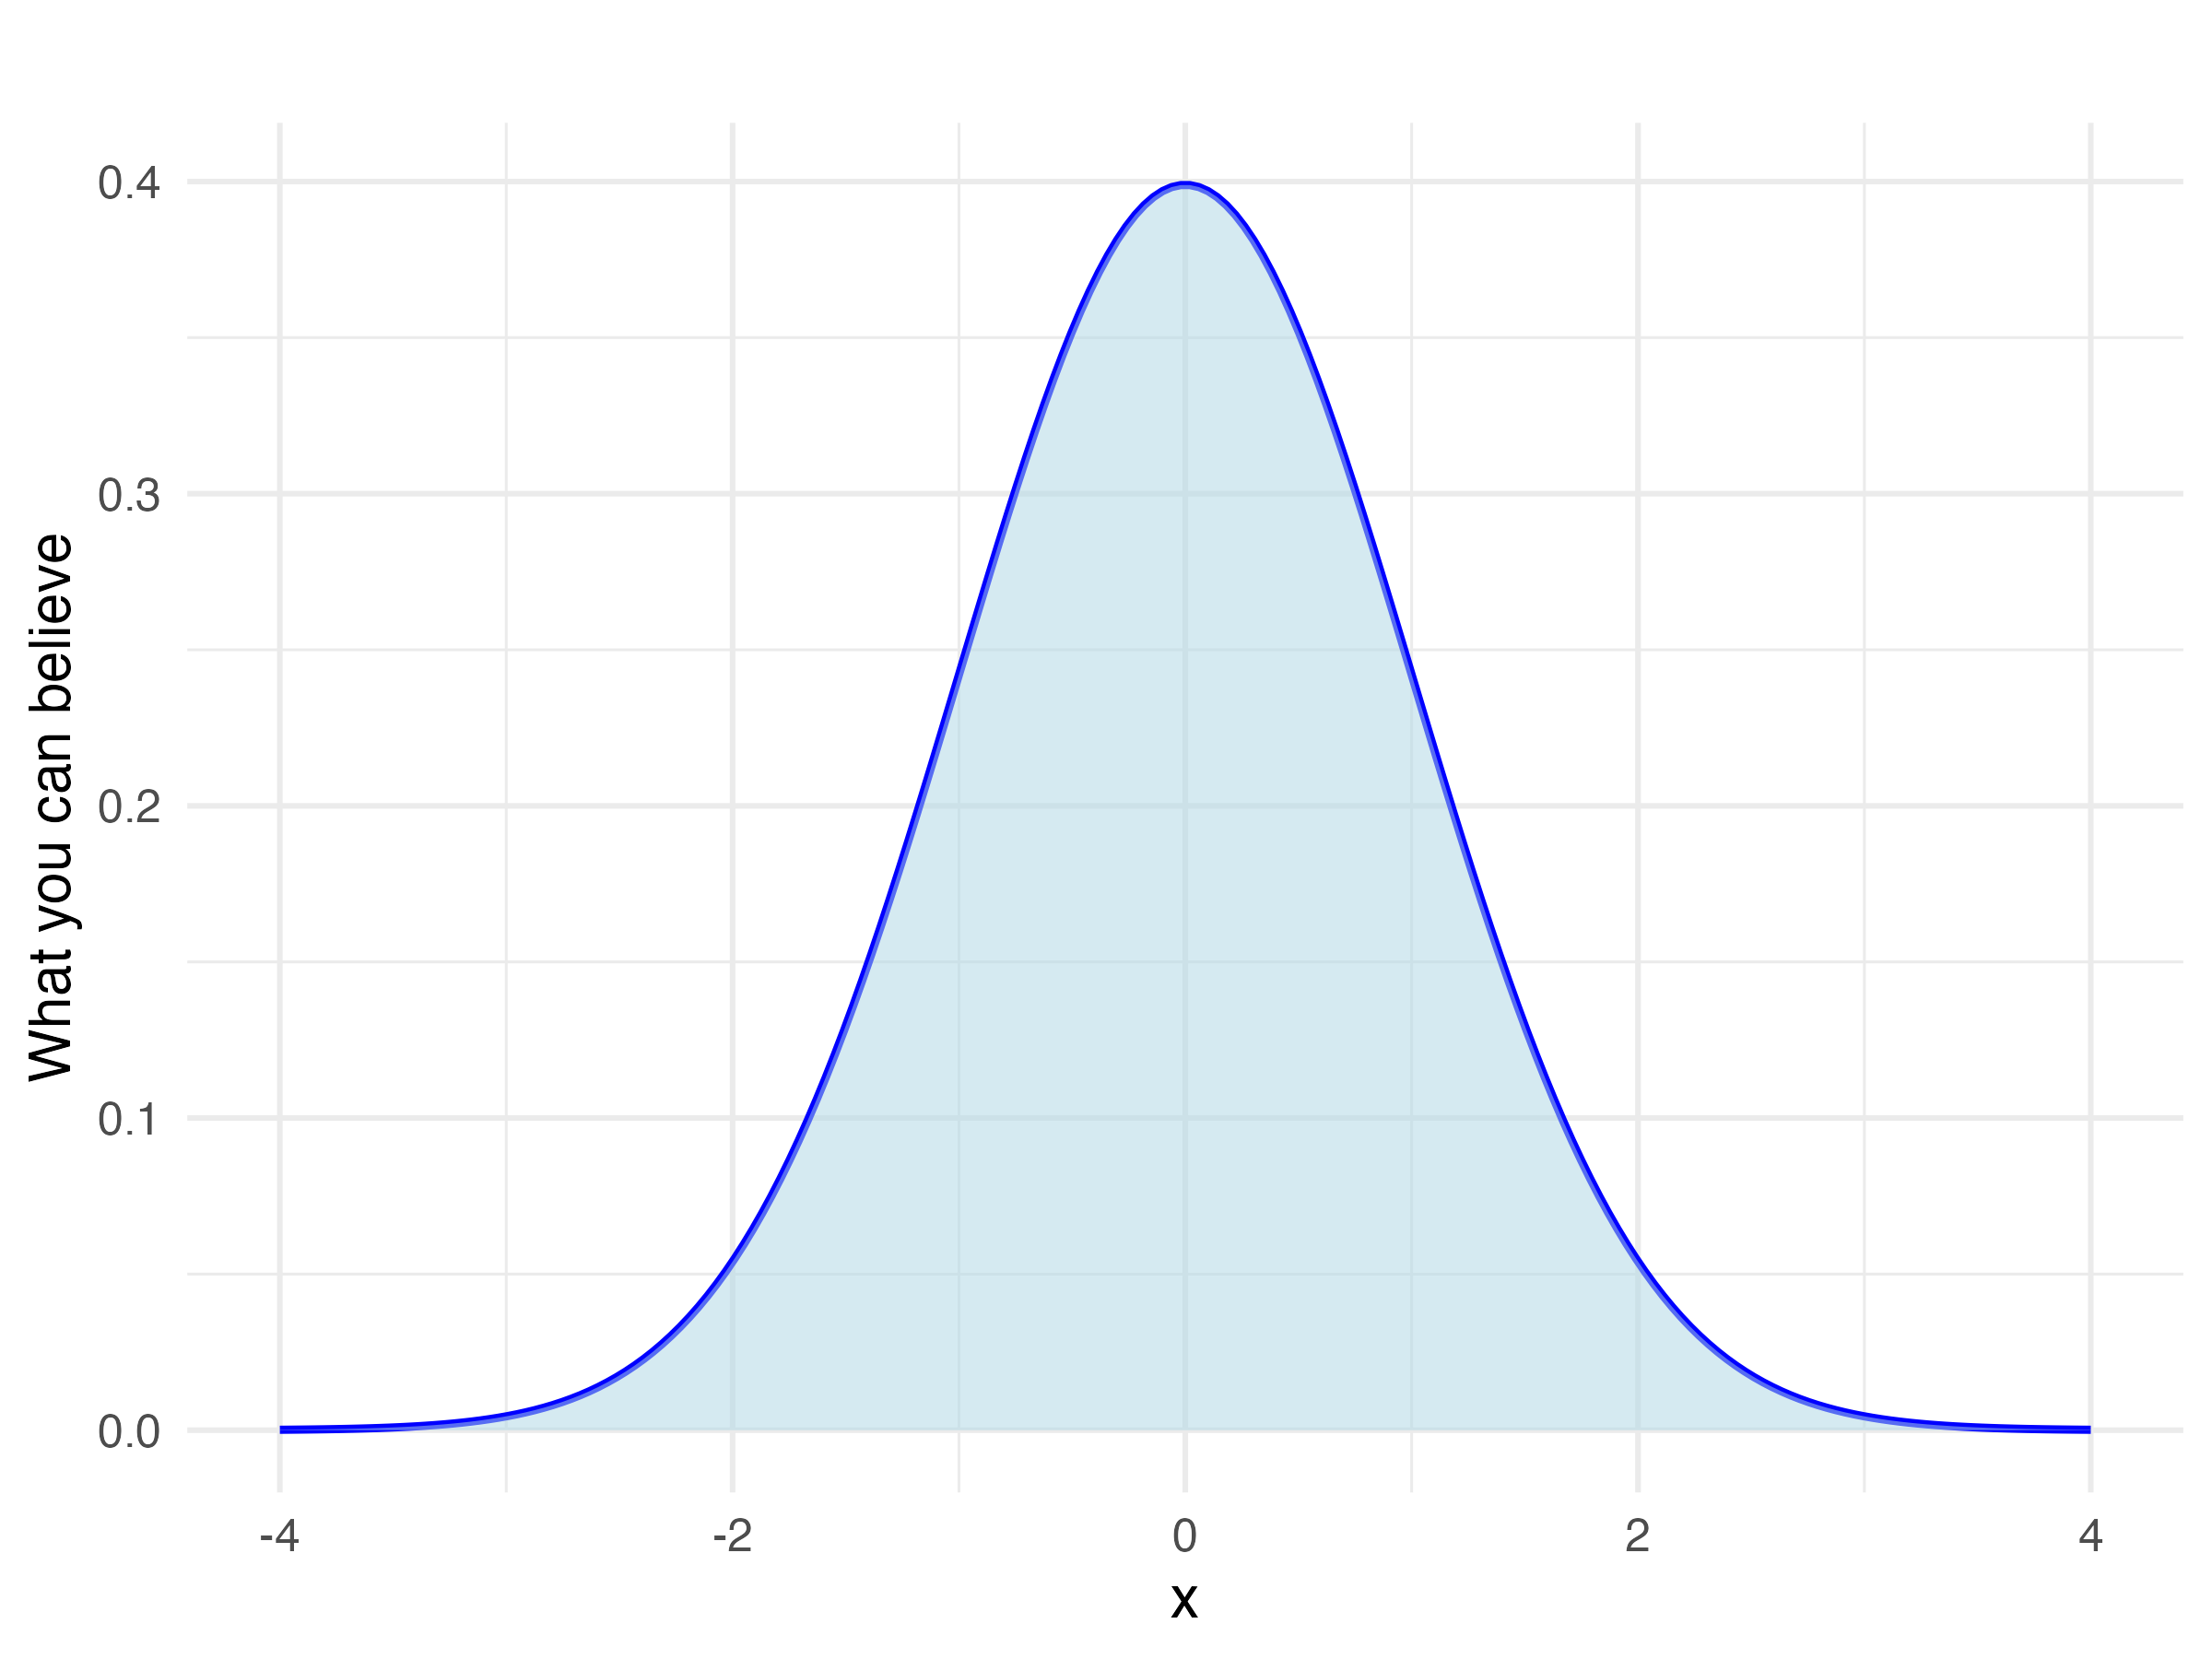
\includegraphics[scale=.35]{figures/example_prior.png}
    \caption{Total ignorance}
    \label{fig:prior}
\end{figure}
\end{frame}

\begin{frame}{GP intuition: Ignorance and neighbors}
\small
\onslide<1-> Now I tell you we see $Y_{obs}=-1$, and $cor(Y^*,Y_{obs})=.8$. Then you believe:\\

\begin{figure}
    \centering
    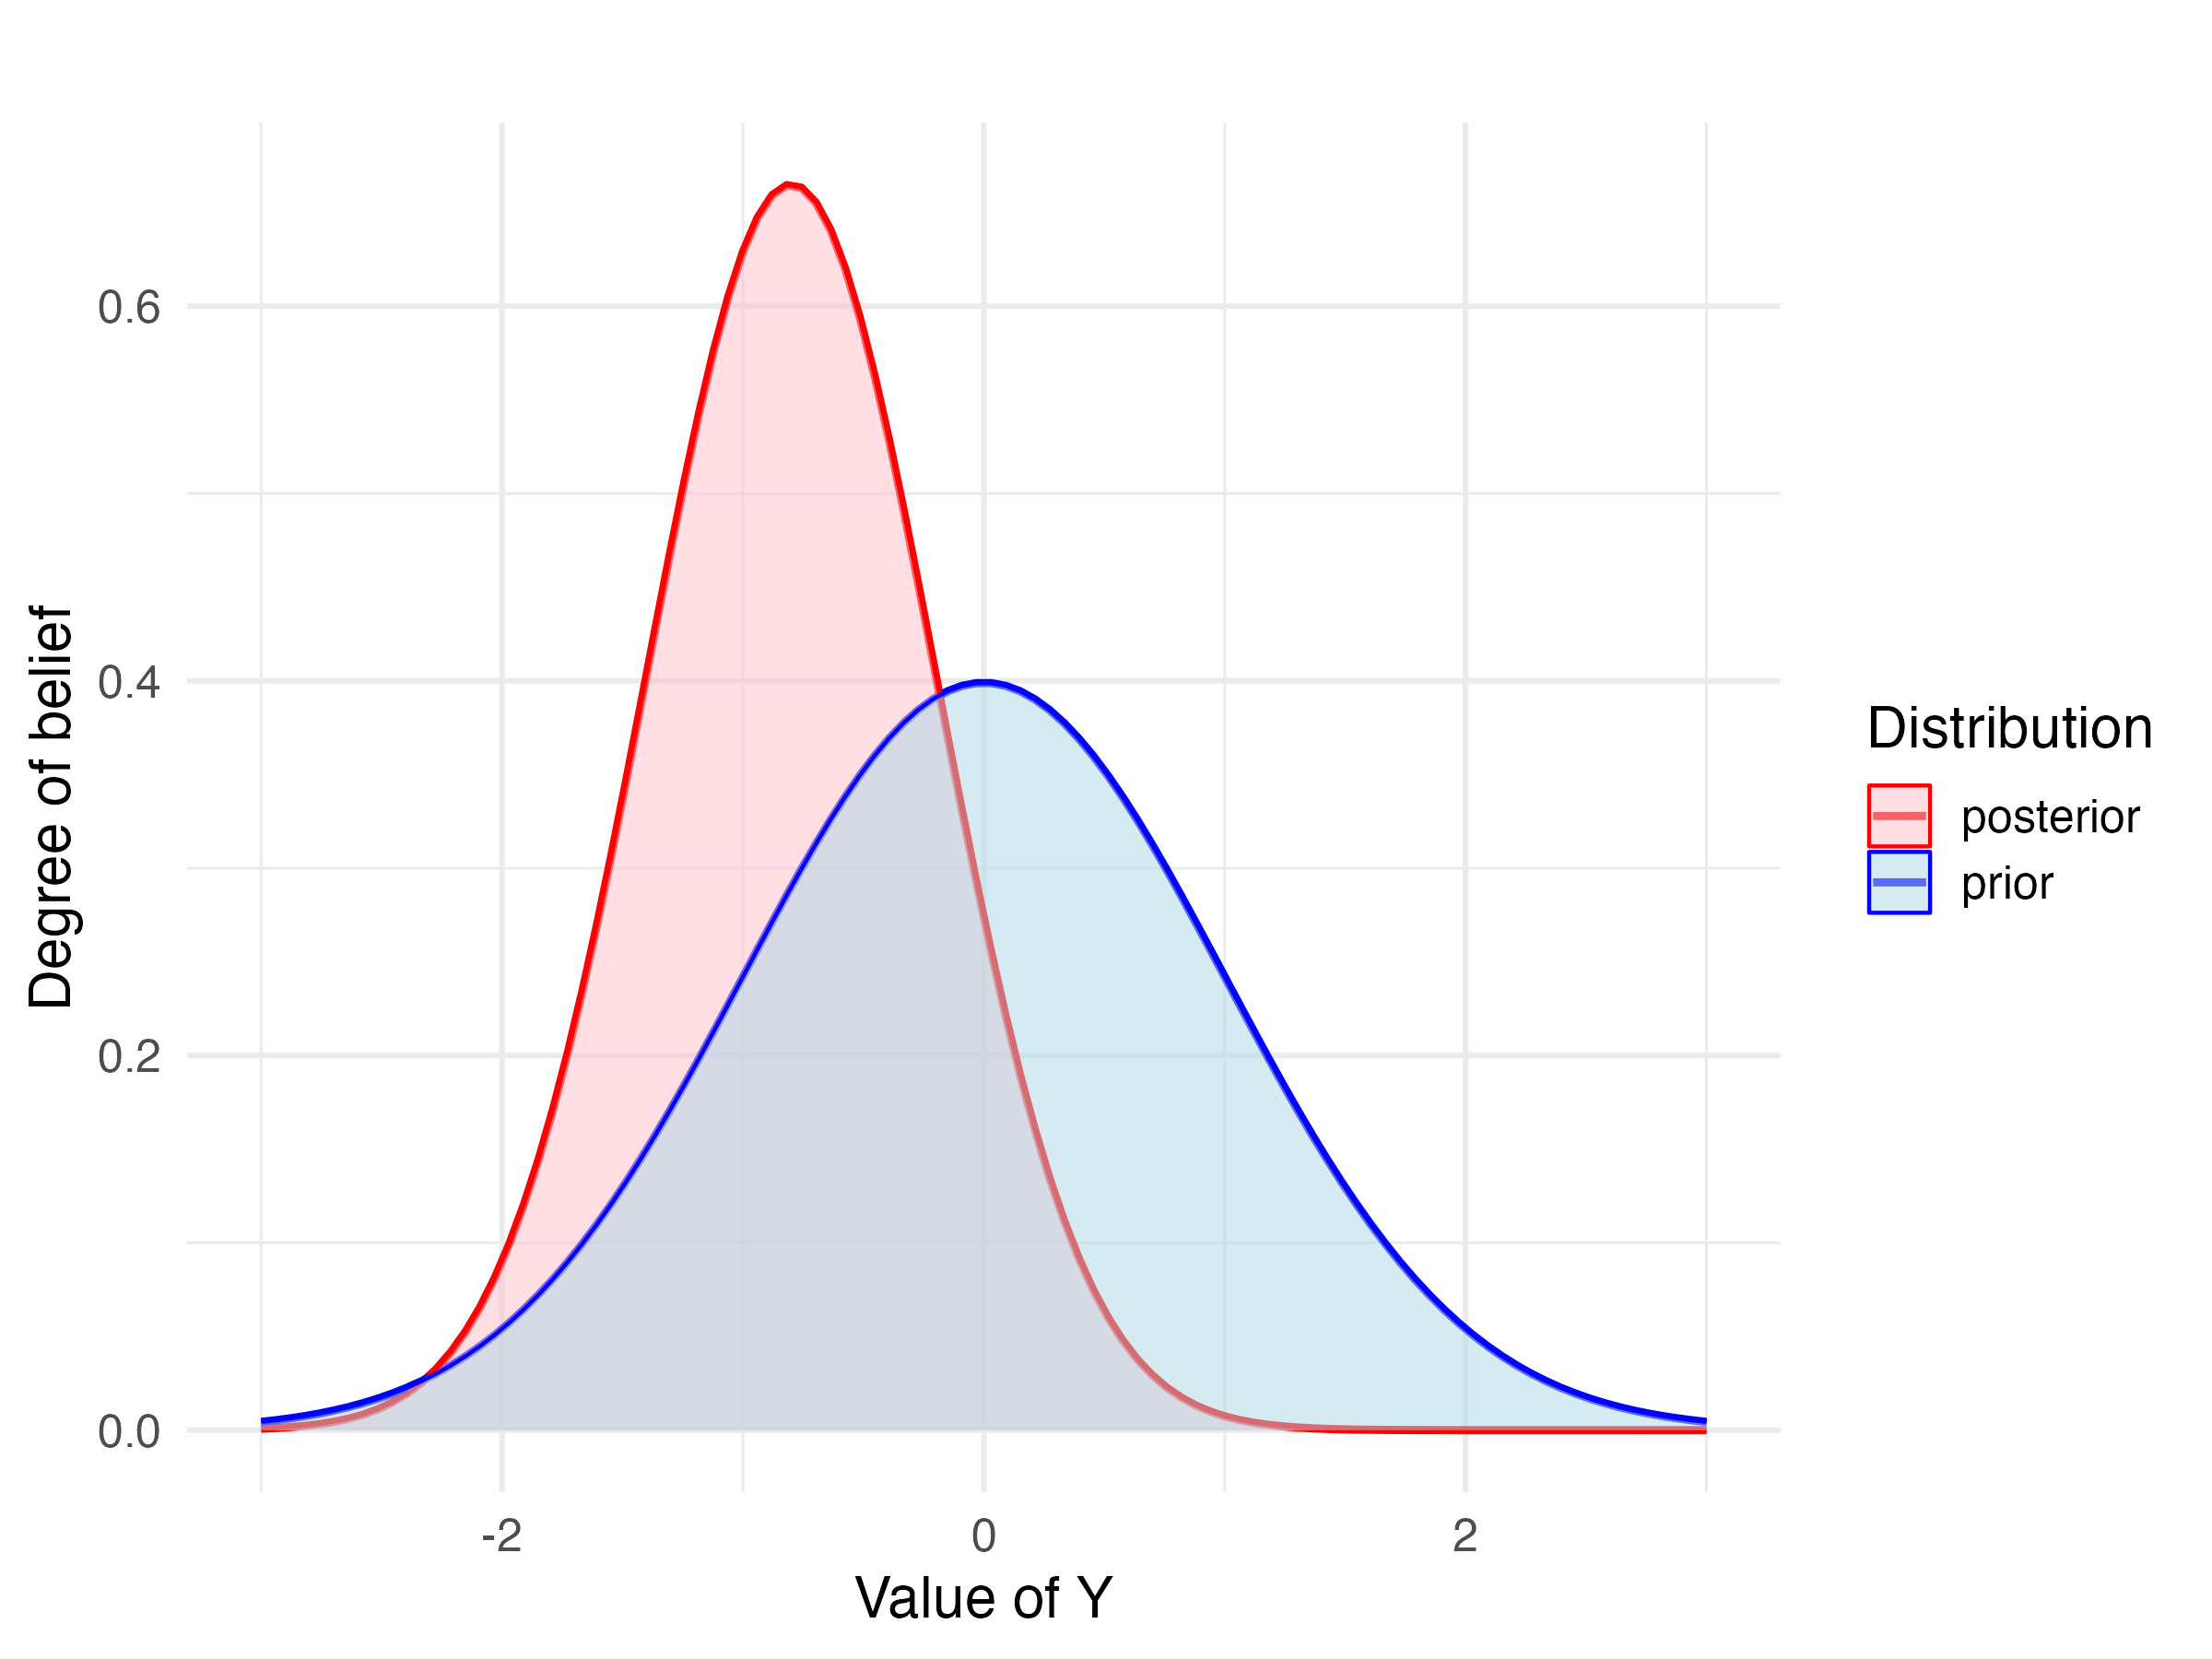
\includegraphics[scale=.35]{figures/example_priorpost.png}
    \caption{Informed ignorance}
    \label{fig:prior}
\end{figure}
\end{frame}

\begin{frame}{GP intuition: Ignorance and neighbors}
\onslide<1-> Now suppose you have numerous observations of $\{X_i,Y_i\}_i^N$. \\
\bigskip
\onslide<2-> Big idea: observations nearer each other in $X$ should have similar $Y$, whatever the values: \\
\begin{itemize}
    \item That is, $cov(Y_i,Y_j)$ larger when $X_i$ nearer $X_j$. 
    \item E.g.,   $cov(Y_i,Y_j) = k(X_i,X_j) = e^{-\frac{||X_i-X_j||^2}{b}}$
\end{itemize}   
% \begin{center}{``Across the datasets you could draw, \textit{units with more similar $X$ will have more similar $Y$}''}\end{center}\\
% \bigskip
% \onslide<5-> Now, after seeing the $Y$s of nearby observations, we can ask where that leaves us: $Y$ at some $X=x^*$,\\
\bigskip
\onslide<3-> At values of $x^*$ near to observed points, the high covariance with observed $Y$s \textcolor{Blue}{improves our guess about $Y^*$}. \\
\bigskip
\onslide<4-> At values of $x^*$ far from observed points, low covariance of observed outcomes with $Y^*$ \textcolor{Red}{leaves us more uncertain about $p(Y^*)$}.
\end{frame}

\begin{frame}{Inferences given a few observations}
\onslide<1-> Given GP assumptions and 5 observations of $\{X_i,Y_i\}$, ask for predictions at any $X$:

\begin{figure}
    \centering
    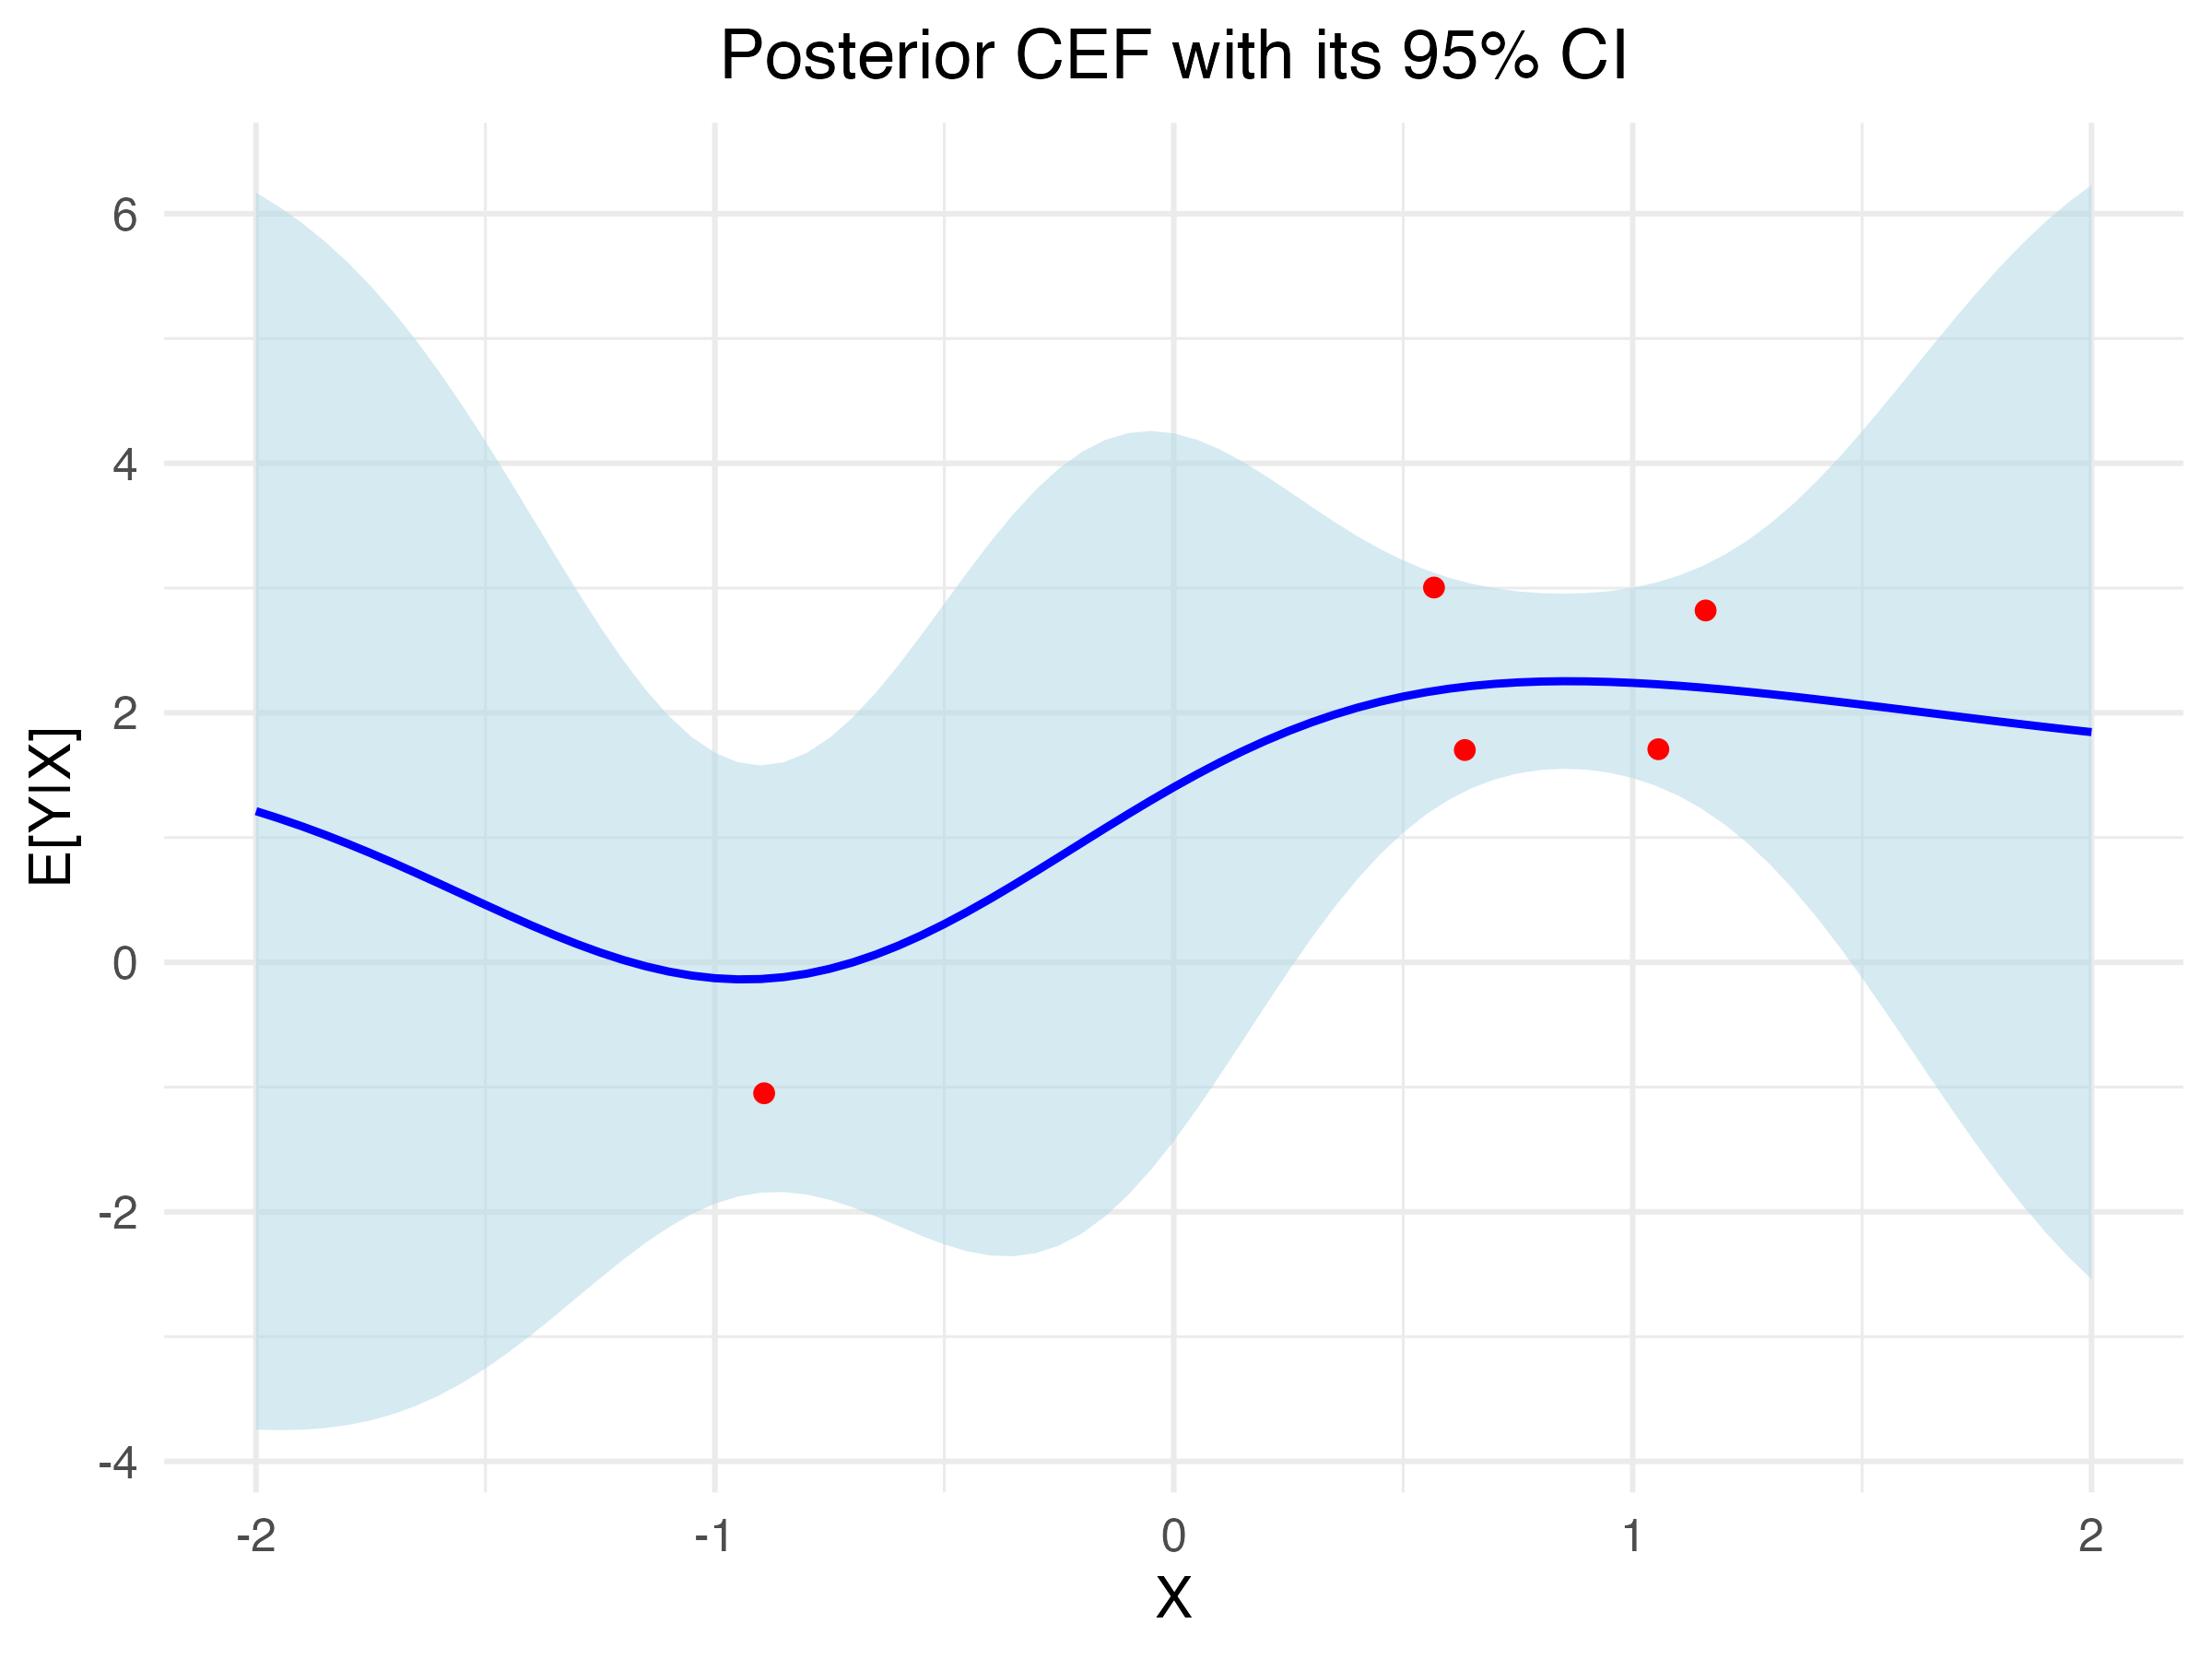
\includegraphics[scale=.45]{figures/example_with_x.png}
    %\caption{Predictions across $X$, given a few observations}
    \label{fig:prior}
\end{figure}
\end{frame}

\begin{frame}{Written out,}
\footnotesize
\begin{enumerate}
    \item<1-> $Y \sim \mathcal{N}(\mu, \Sigma)$, deferring how $\mu$ and  $\Sigma$ will be determined.
    \item<2-> Choose a kernel function $k(\cdot, \cdot)$, with $cov(Y_i,Y_j)=\sigma_y k(X_i,X_j)$.  This can be given a particular form, such as $k(X_i,X_j)= exp(-||X_i-X_j||^2/b)$. 
    \item<3-> Consider the kernel matrix $\K$, containing all the pairwise kernel evaluations, i.e. $\K_{i,j}=k(X_i,X_j)$. 
    \item<4-> Then,
        \[ Y|X \sim \mathcal{N}(\mu,\sigma_y \K) \] 
       
    \item<5-> That model \textit{goes through every point}, but we expect noise:
    $$Y|X \sim \mathcal{N}(\mu,\sigma_y(\K+\sigma^2 I))$$
    \item<6-> After centering and scaling $Y$ we can  use $\mu=0$ and $\sigma_y=1$,
            $$Y|X \sim \mathcal{N}(0,\K+\sigma^2 I)$$
    \item<7-> ``Conditioning on the observations'', beliefs about the distribution of test points ($Y^*$) is
    \begin{align}\label{eq.main}
    Y^* \sim \mathcal{N}(\K_* \underbrace{(\K+\sigma^2 I)^{-1}Y}_{\text{coefs.}}, \underbrace{\K_{*,*}+\sigma^2 I}_{\text{prior var}} - \underbrace{\K_*^{\top} (\K+\sigma^2 I)^{-1}\K_*}_{ \text{reduction due to data}})
    \end{align}
\end{enumerate}
\end{frame}

%\begin{frame}{Aside: Uncertainty and extrapolation in 3 models}
%\begin{figure}[hbt!]
%\begin{center}
%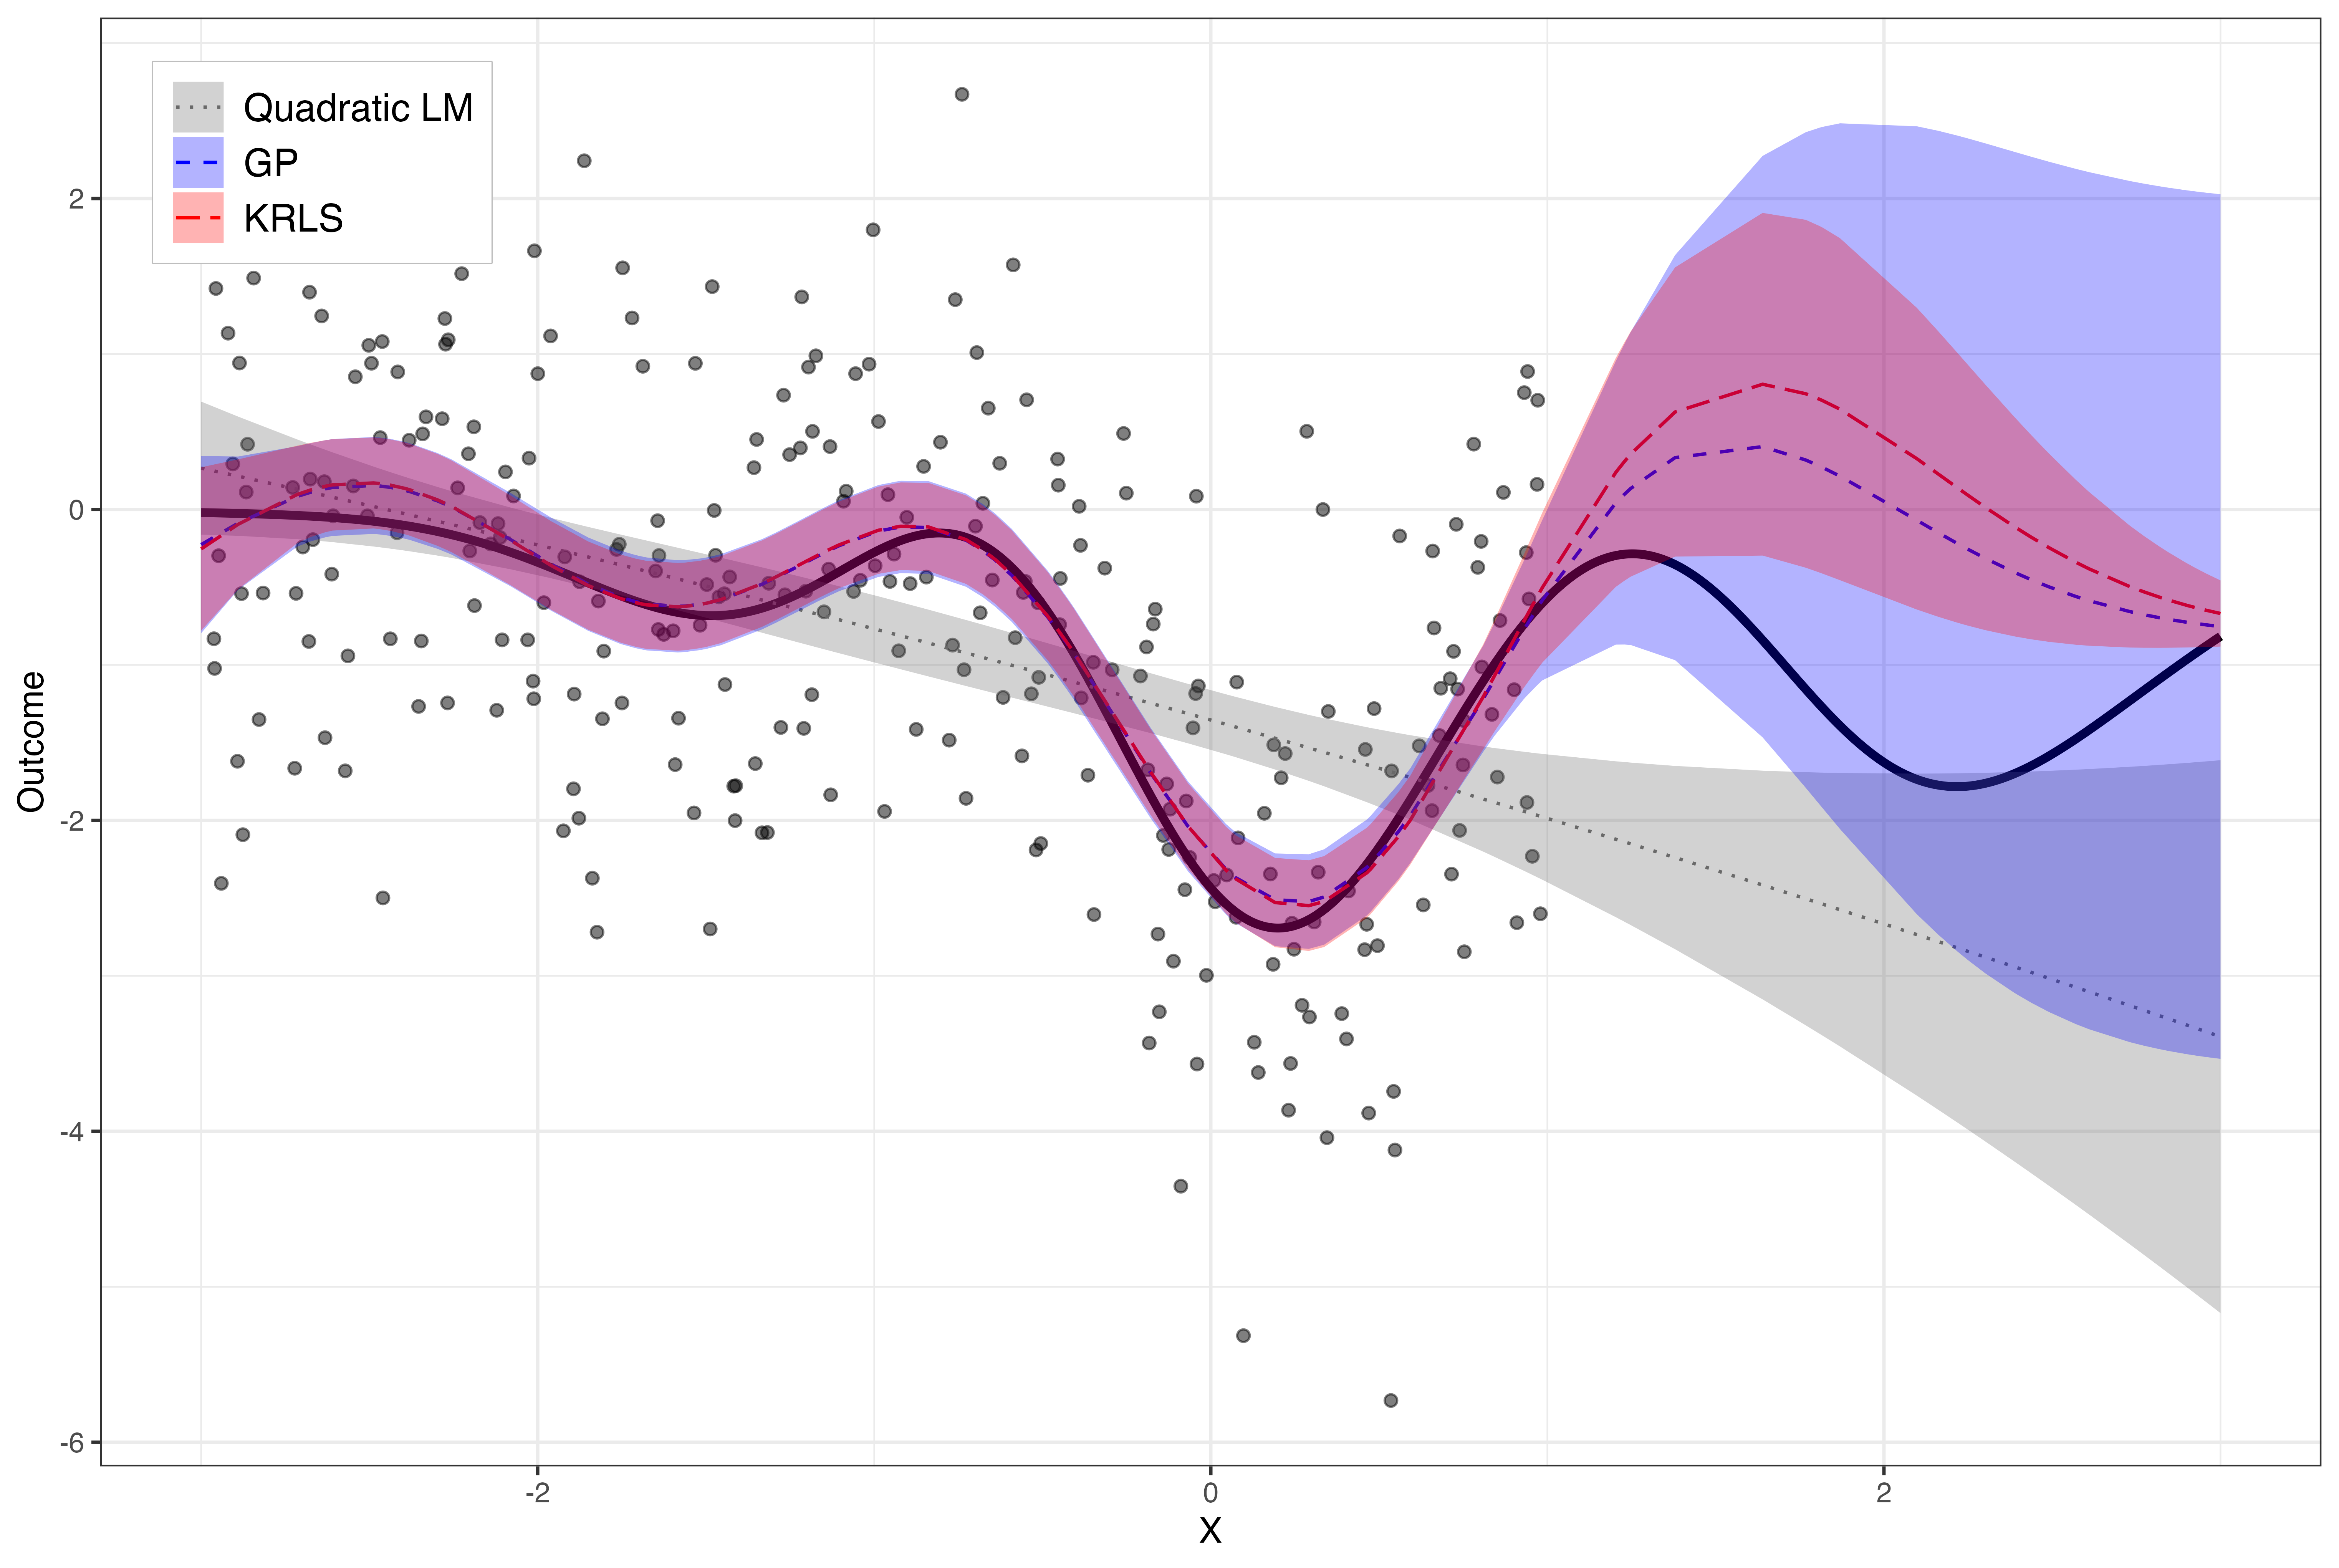
\includegraphics[width=.55\textwidth]{figures/krls_gp_quadratic.png}
%%\caption{Models are fitted on $X$ data between -3 and 1, then extrapolated over $X$ between 1 and 3. The solid line shows the true function (drawn at random), while dashed/dotted lines indicate each model's estimated CEF. Bands indicate 95\% CIs for the CEFs.}
%\label{fig:krls_gp_quadratic}
%\end{center}
%\end{figure}
%\footnotesize
%\begin{itemize}
%\item<2-> In linear model, $var(\E[Y^*|X_i]) \propto X_i^{2} Var(\beta)$, but is silent on model uncertainty
%\item<3-> GP and kernel ridge regression/least squares (KRLS) have same CEF/\textit{maximum a posteriori}, including the ``return to mean''
%\item<4-> But with GP the uncertainty shows our ignorance farther from the data
%\end{itemize}
%\end{frame}



\begin{frame}{Case 3: Regression Discontinuity}
%\onslide<1-> The RD design is widely used where possible for credible local inference. \\
\bigskip
        % \begin{itemize}
        %     \item Continuous $\E[Y(d)|Z=c]$
        %     \item Local randomization view:  $$\{ Y_{1}, Y_0 \} \independent D|Z=c$$
        % \end{itemize}
        % \vspace{1em}
\onslide<1-> RD requires estimating to the edge of the data, or slightly past it: \\
\small
         \begin{itemize}
             \item  $\widehat{Y(0)}_{Z=c}$: Train $\E[Y(0)|Z]$ on $Z<c$ and predict at $Z=c$ 
             \item  $\widehat{Y(1)}_{Z=c}$: Train $\E[Y(1)|Z]$ on $Z>c$ and predict at $Z=c$
 \end{itemize}
 \begin{align*}
   \hat{\tau} &= \widehat{Y(1)}_{Z=c} - \widehat{Y(0)}_{Z=c} \\
    \widehat{Var}(\hat{\tau}) &=  \widehat{Var}(\widehat{Y(1)}_{Z=c}) + \widehat{Var}(\widehat{Y(0)}_{Z=c})
\end{align*}
\begin{itemize}
\item<2-> Easy to implement: In \texttt{GPss} package for \texttt{R};  \href{https://doeunkim.org/gpss/}{http://doeunkim.org/gpss}. 
\item<3-> Does not require large samples for reasoned inference
\end{itemize}
\end{frame}


\begin{frame}{RD: random $Z$ and $Y$, large sample }
\onslide<1-> $\tau=3$ (or $\tau=0$), $N=500$, \texttt{rdrobust} at defaults (robust estimate), \texttt{GPrd} at defaults \\
\begin{figure}[hbt!]
\centering 
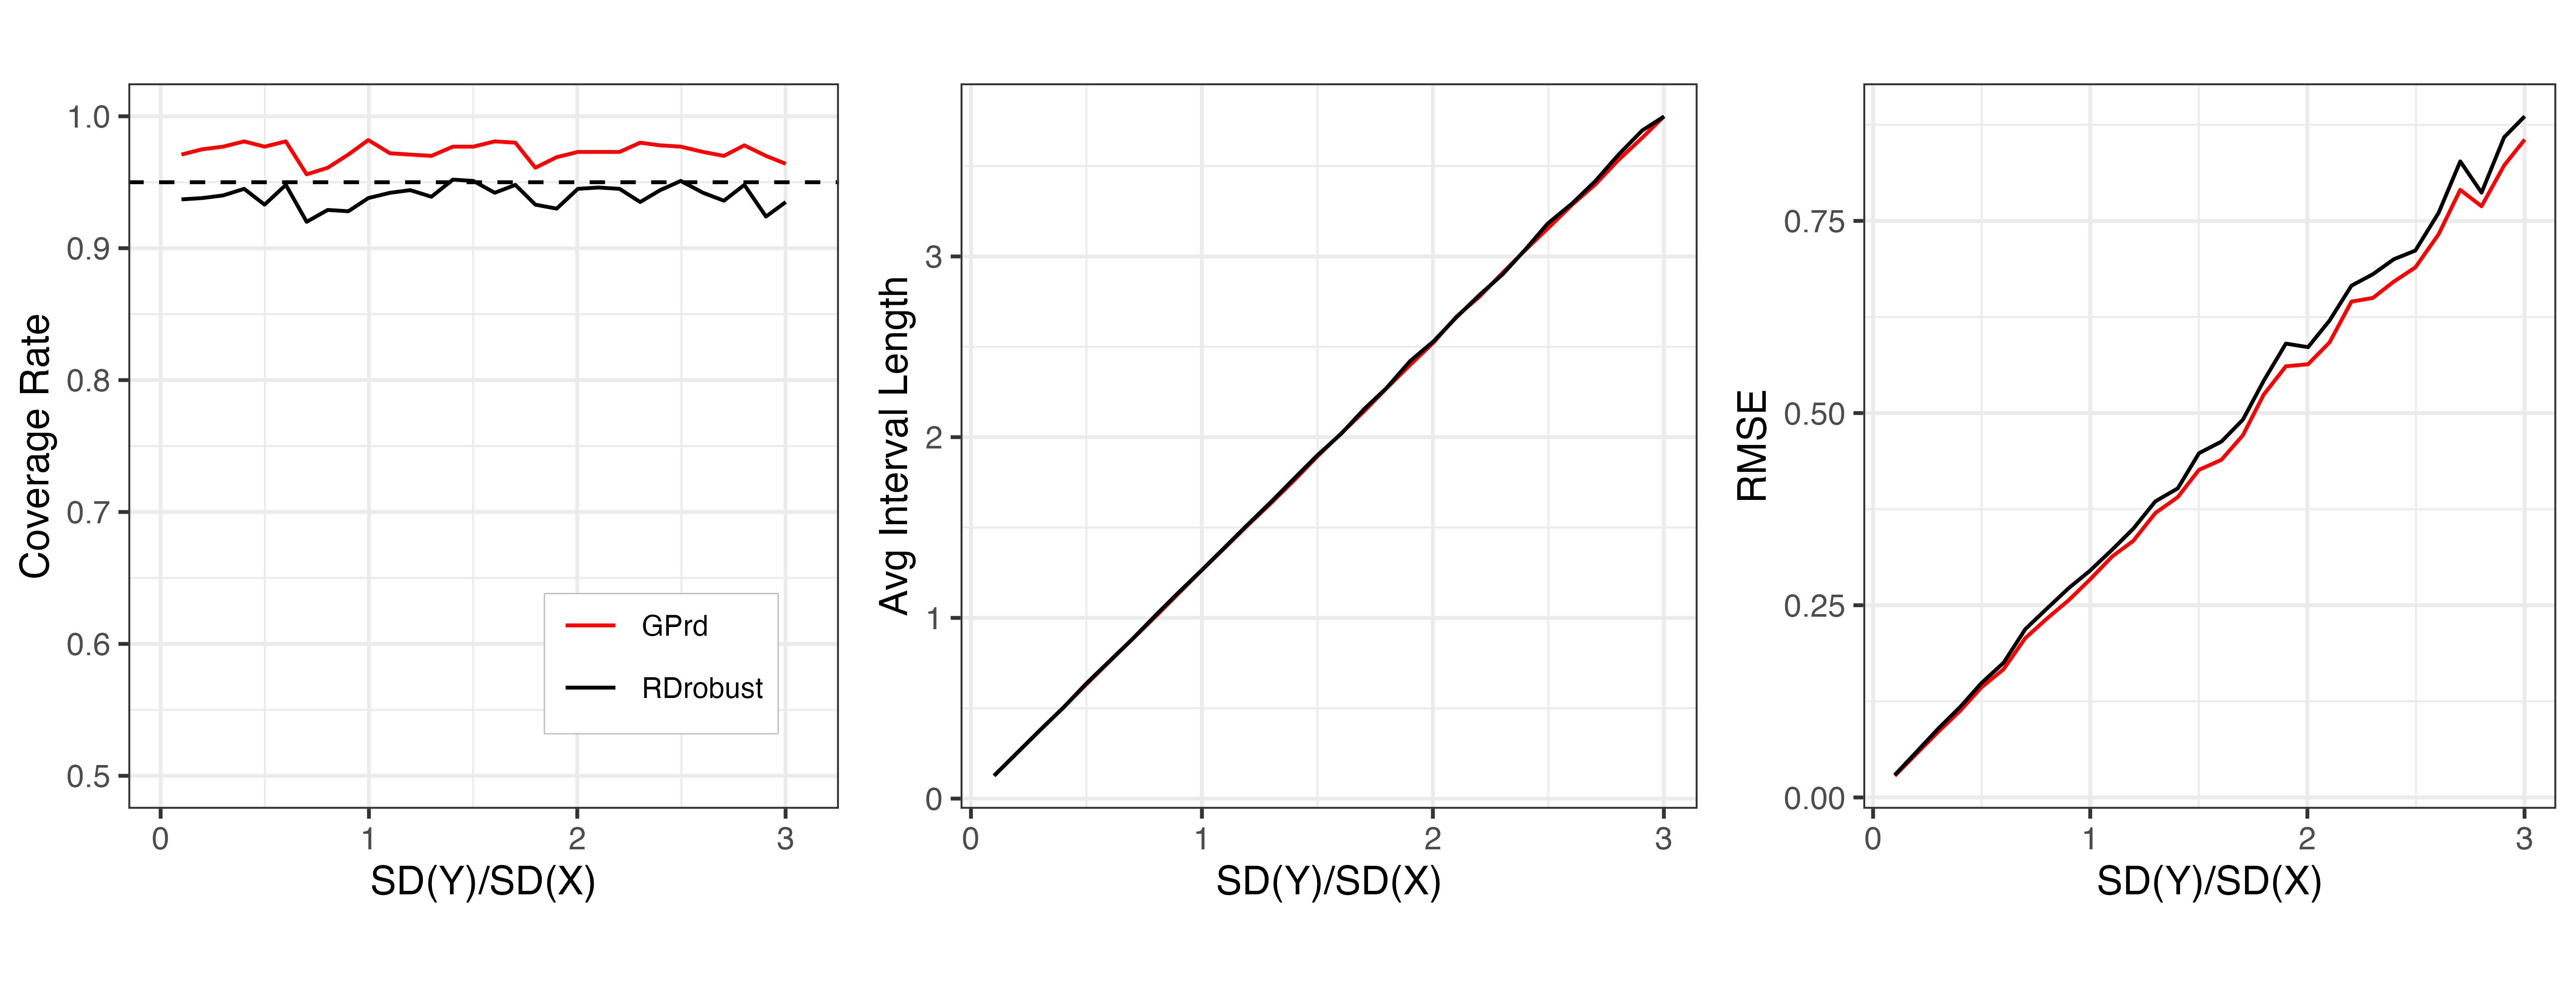
\includegraphics[width=\linewidth]{figures/rdd_totalrandom_n500_effect0_summary.png}\\
\end{figure}
\end{frame}

\begin{frame}{RD: random $Z$ and $Y$, small sample}
\onslide<1-> $\tau=3$ (or $\tau=0$), $N=100$, \texttt{rdrobust} at defaults (robust estimate), \texttt{GPrd} at defaults
\begin{figure}[hbt!]
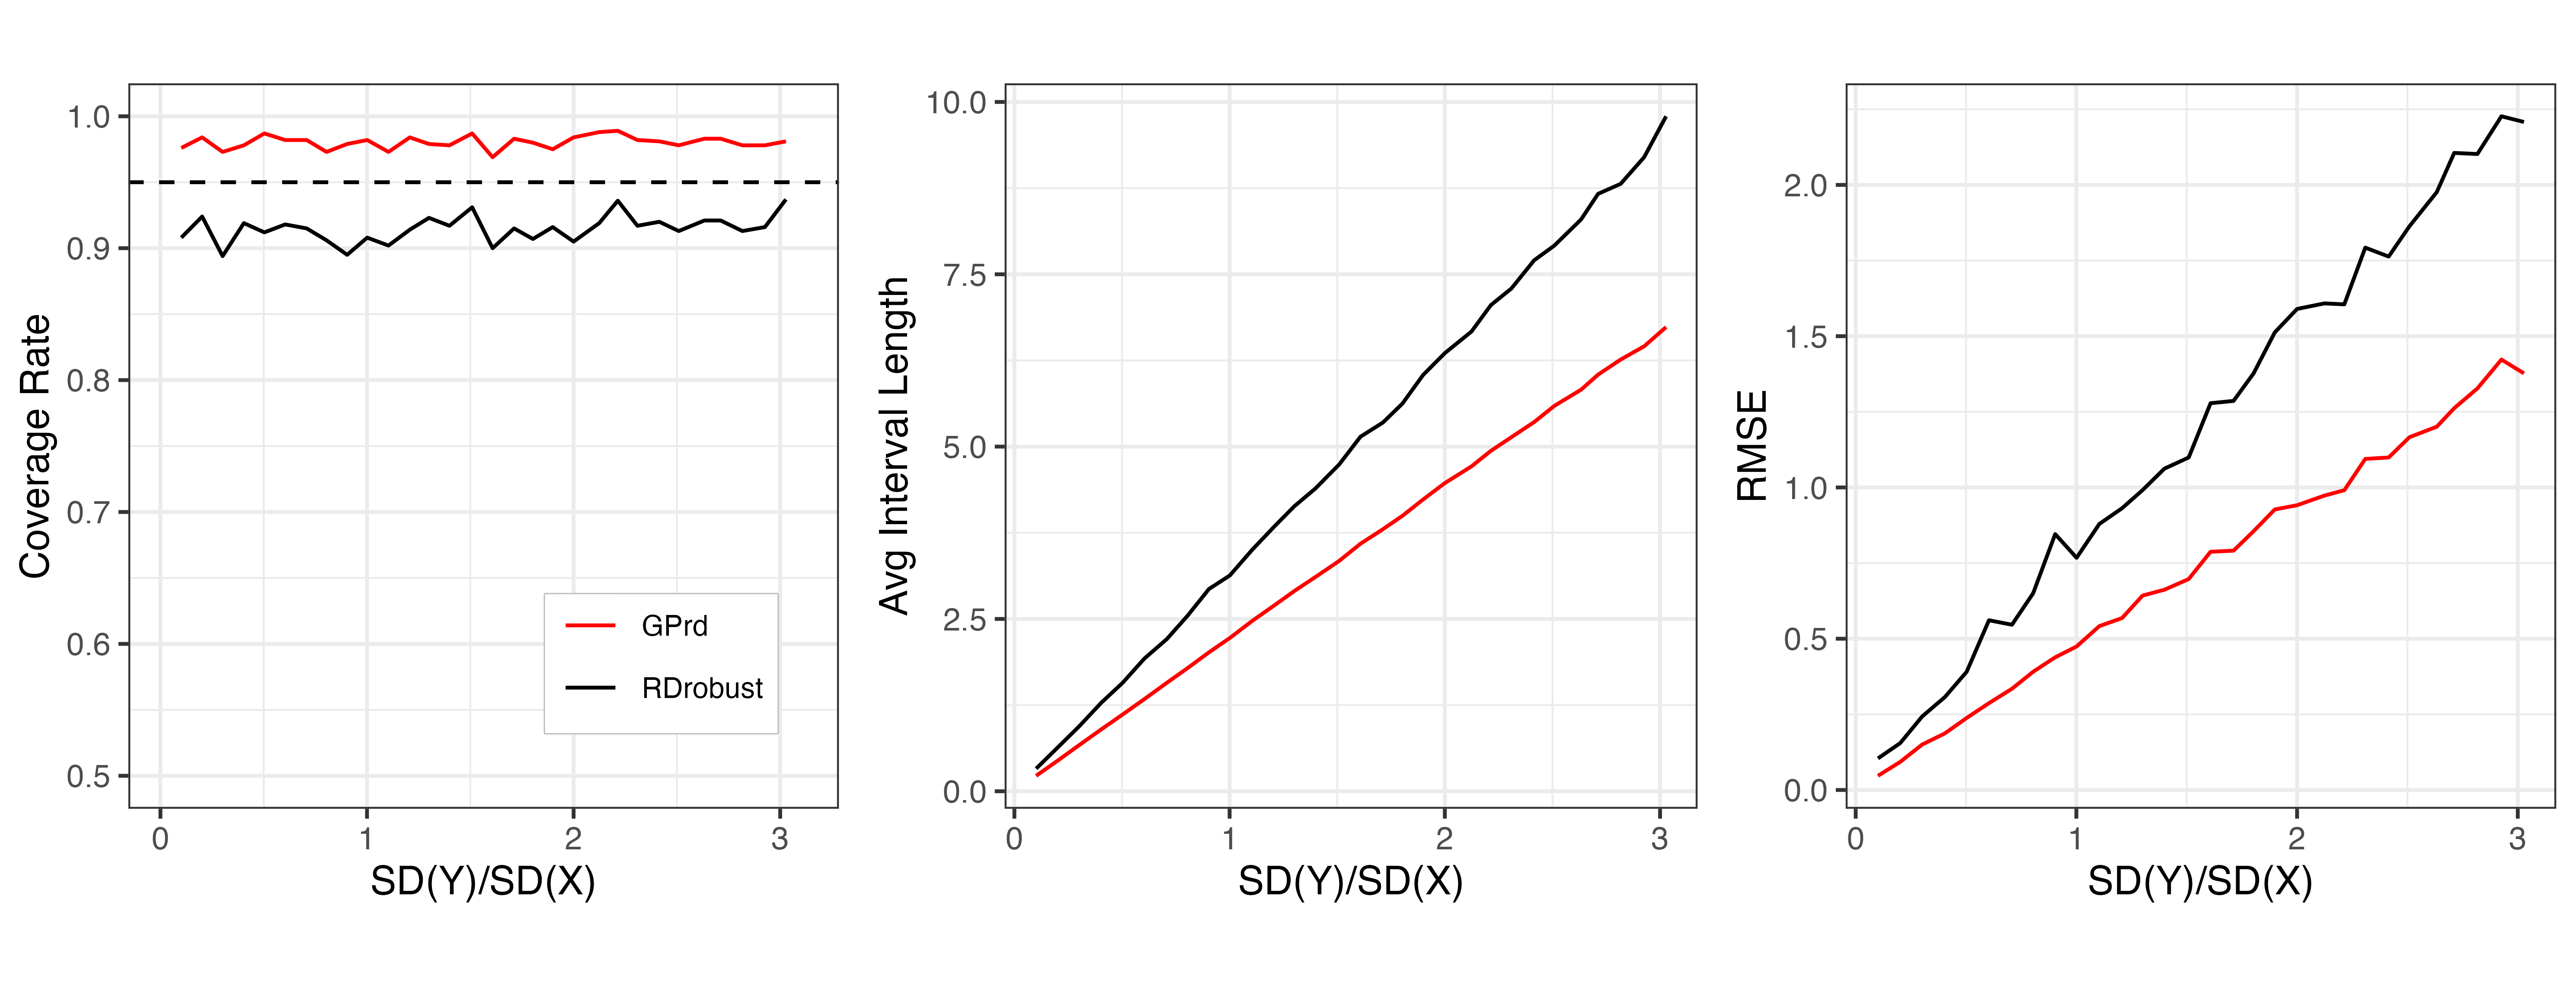
\includegraphics[width=.9\linewidth]{figures/rdd_totalrandom_n100_effect0_summary.png}
\end{figure}
\onslide<2-> Turns out the improved RMSE is the big story, and relates to GP's regularization on each side whereas polynomials can go a little crazy.
%\onslide<2-> (Similar story if you posit a latent variable confounding running variable and outcome)
\end{frame}

% \begin{frame}{Case 3 RD: simulation with random $Z$ and $Y$ ($\tau = 3$)}
% \begin{center}
%     \begin{figure}[hbt!]
%     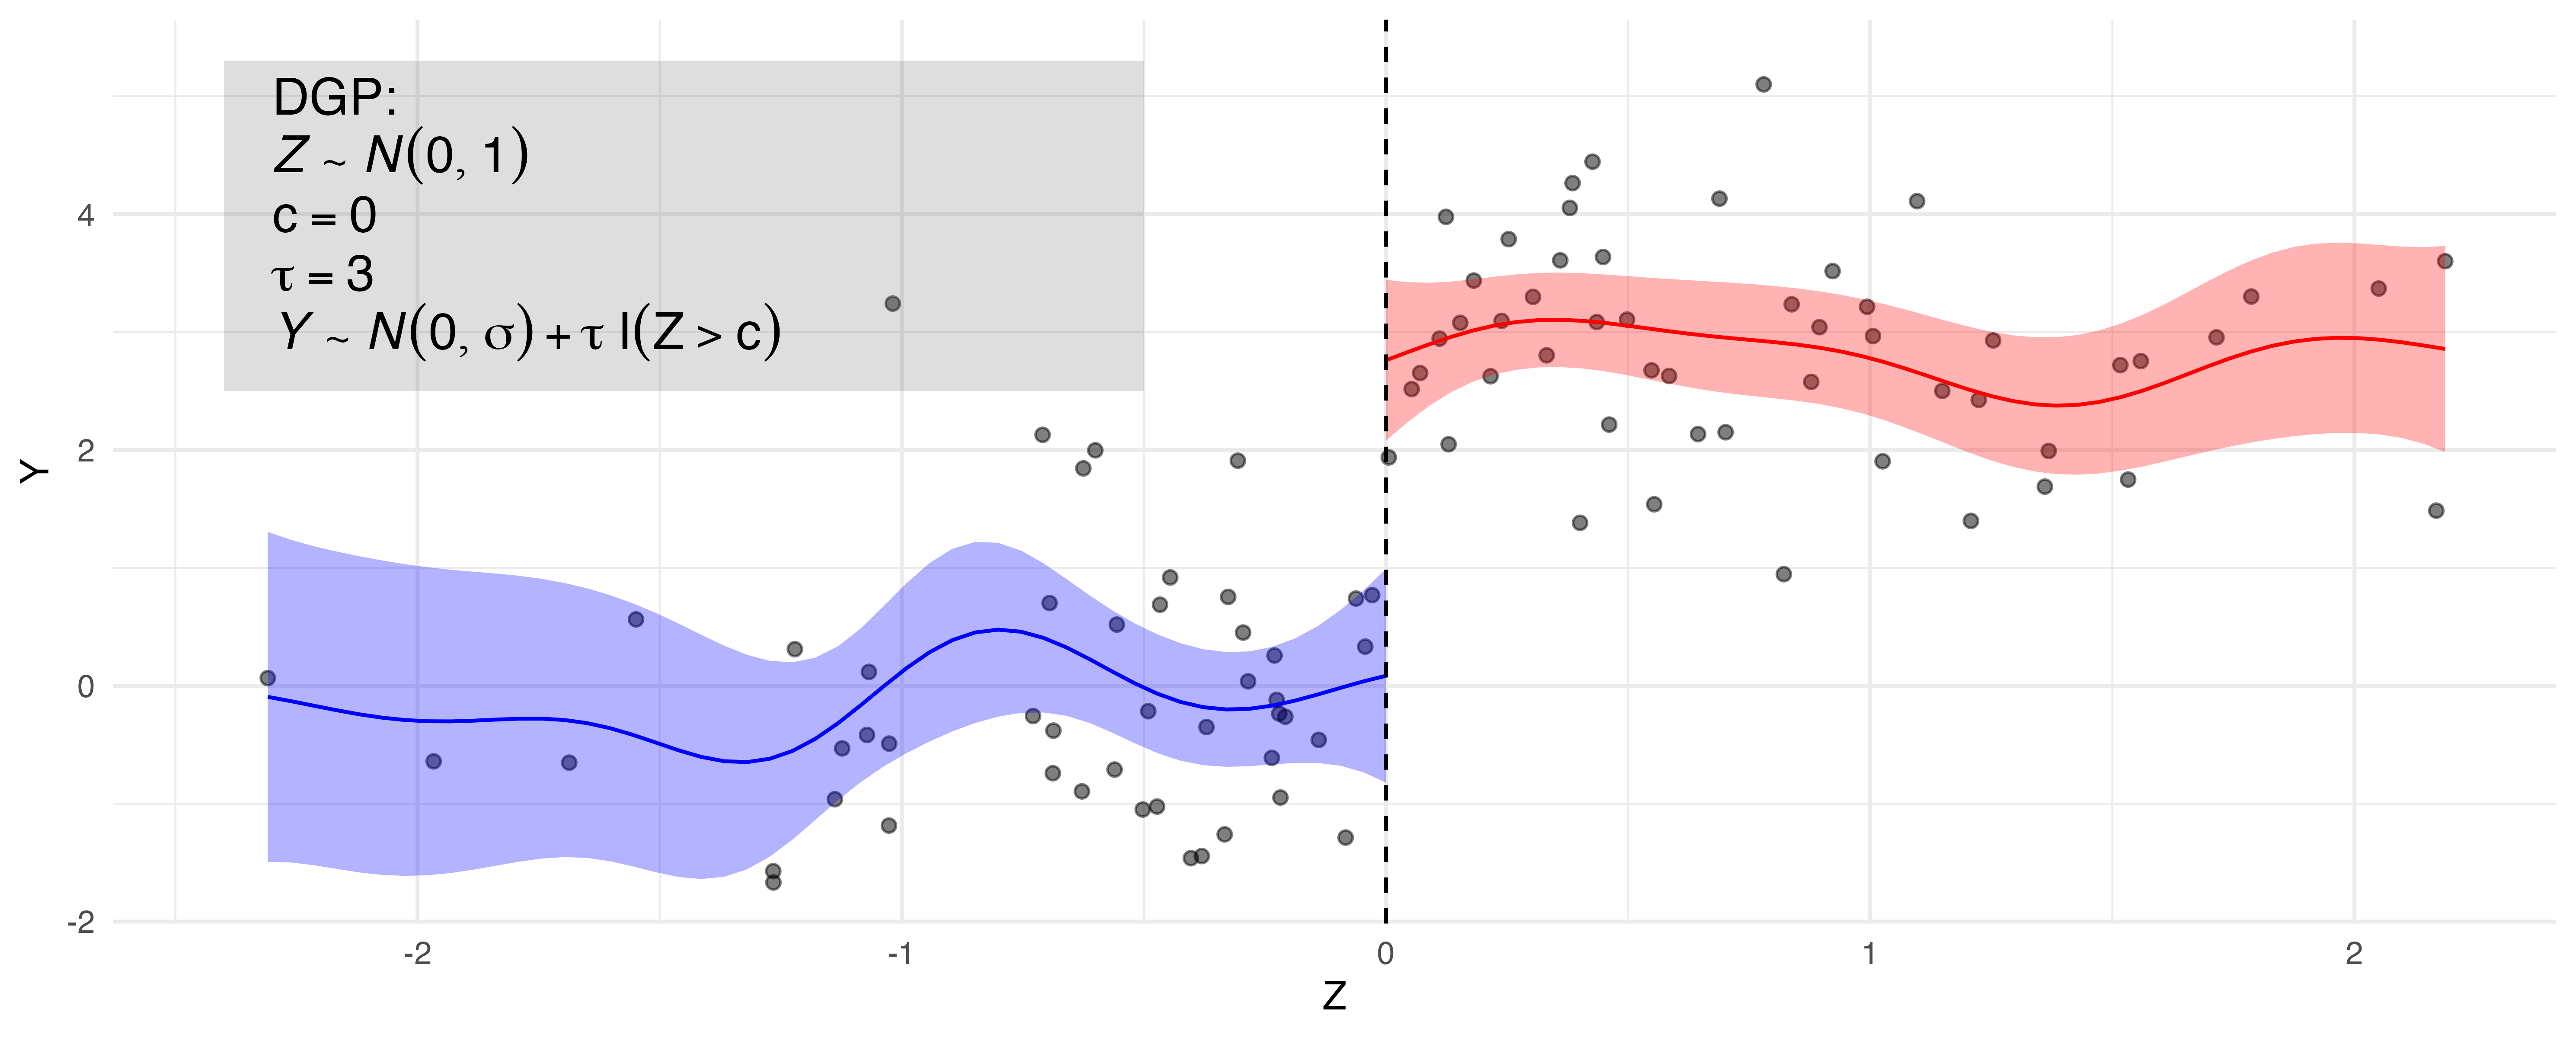
\includegraphics[width=\linewidth]{figures/rdd_sample_tau3.png}
%     \end{figure}
% \end{center}
% \end{frame}

% \begin{frame}{Case 3 RD: simulation with random $Z$ and $Y$ ($\tau = 3$)}
% \vspace{-1.5em}
% \begin{center}
% \end{center}
%     \begin{figure}[hbt!]
%     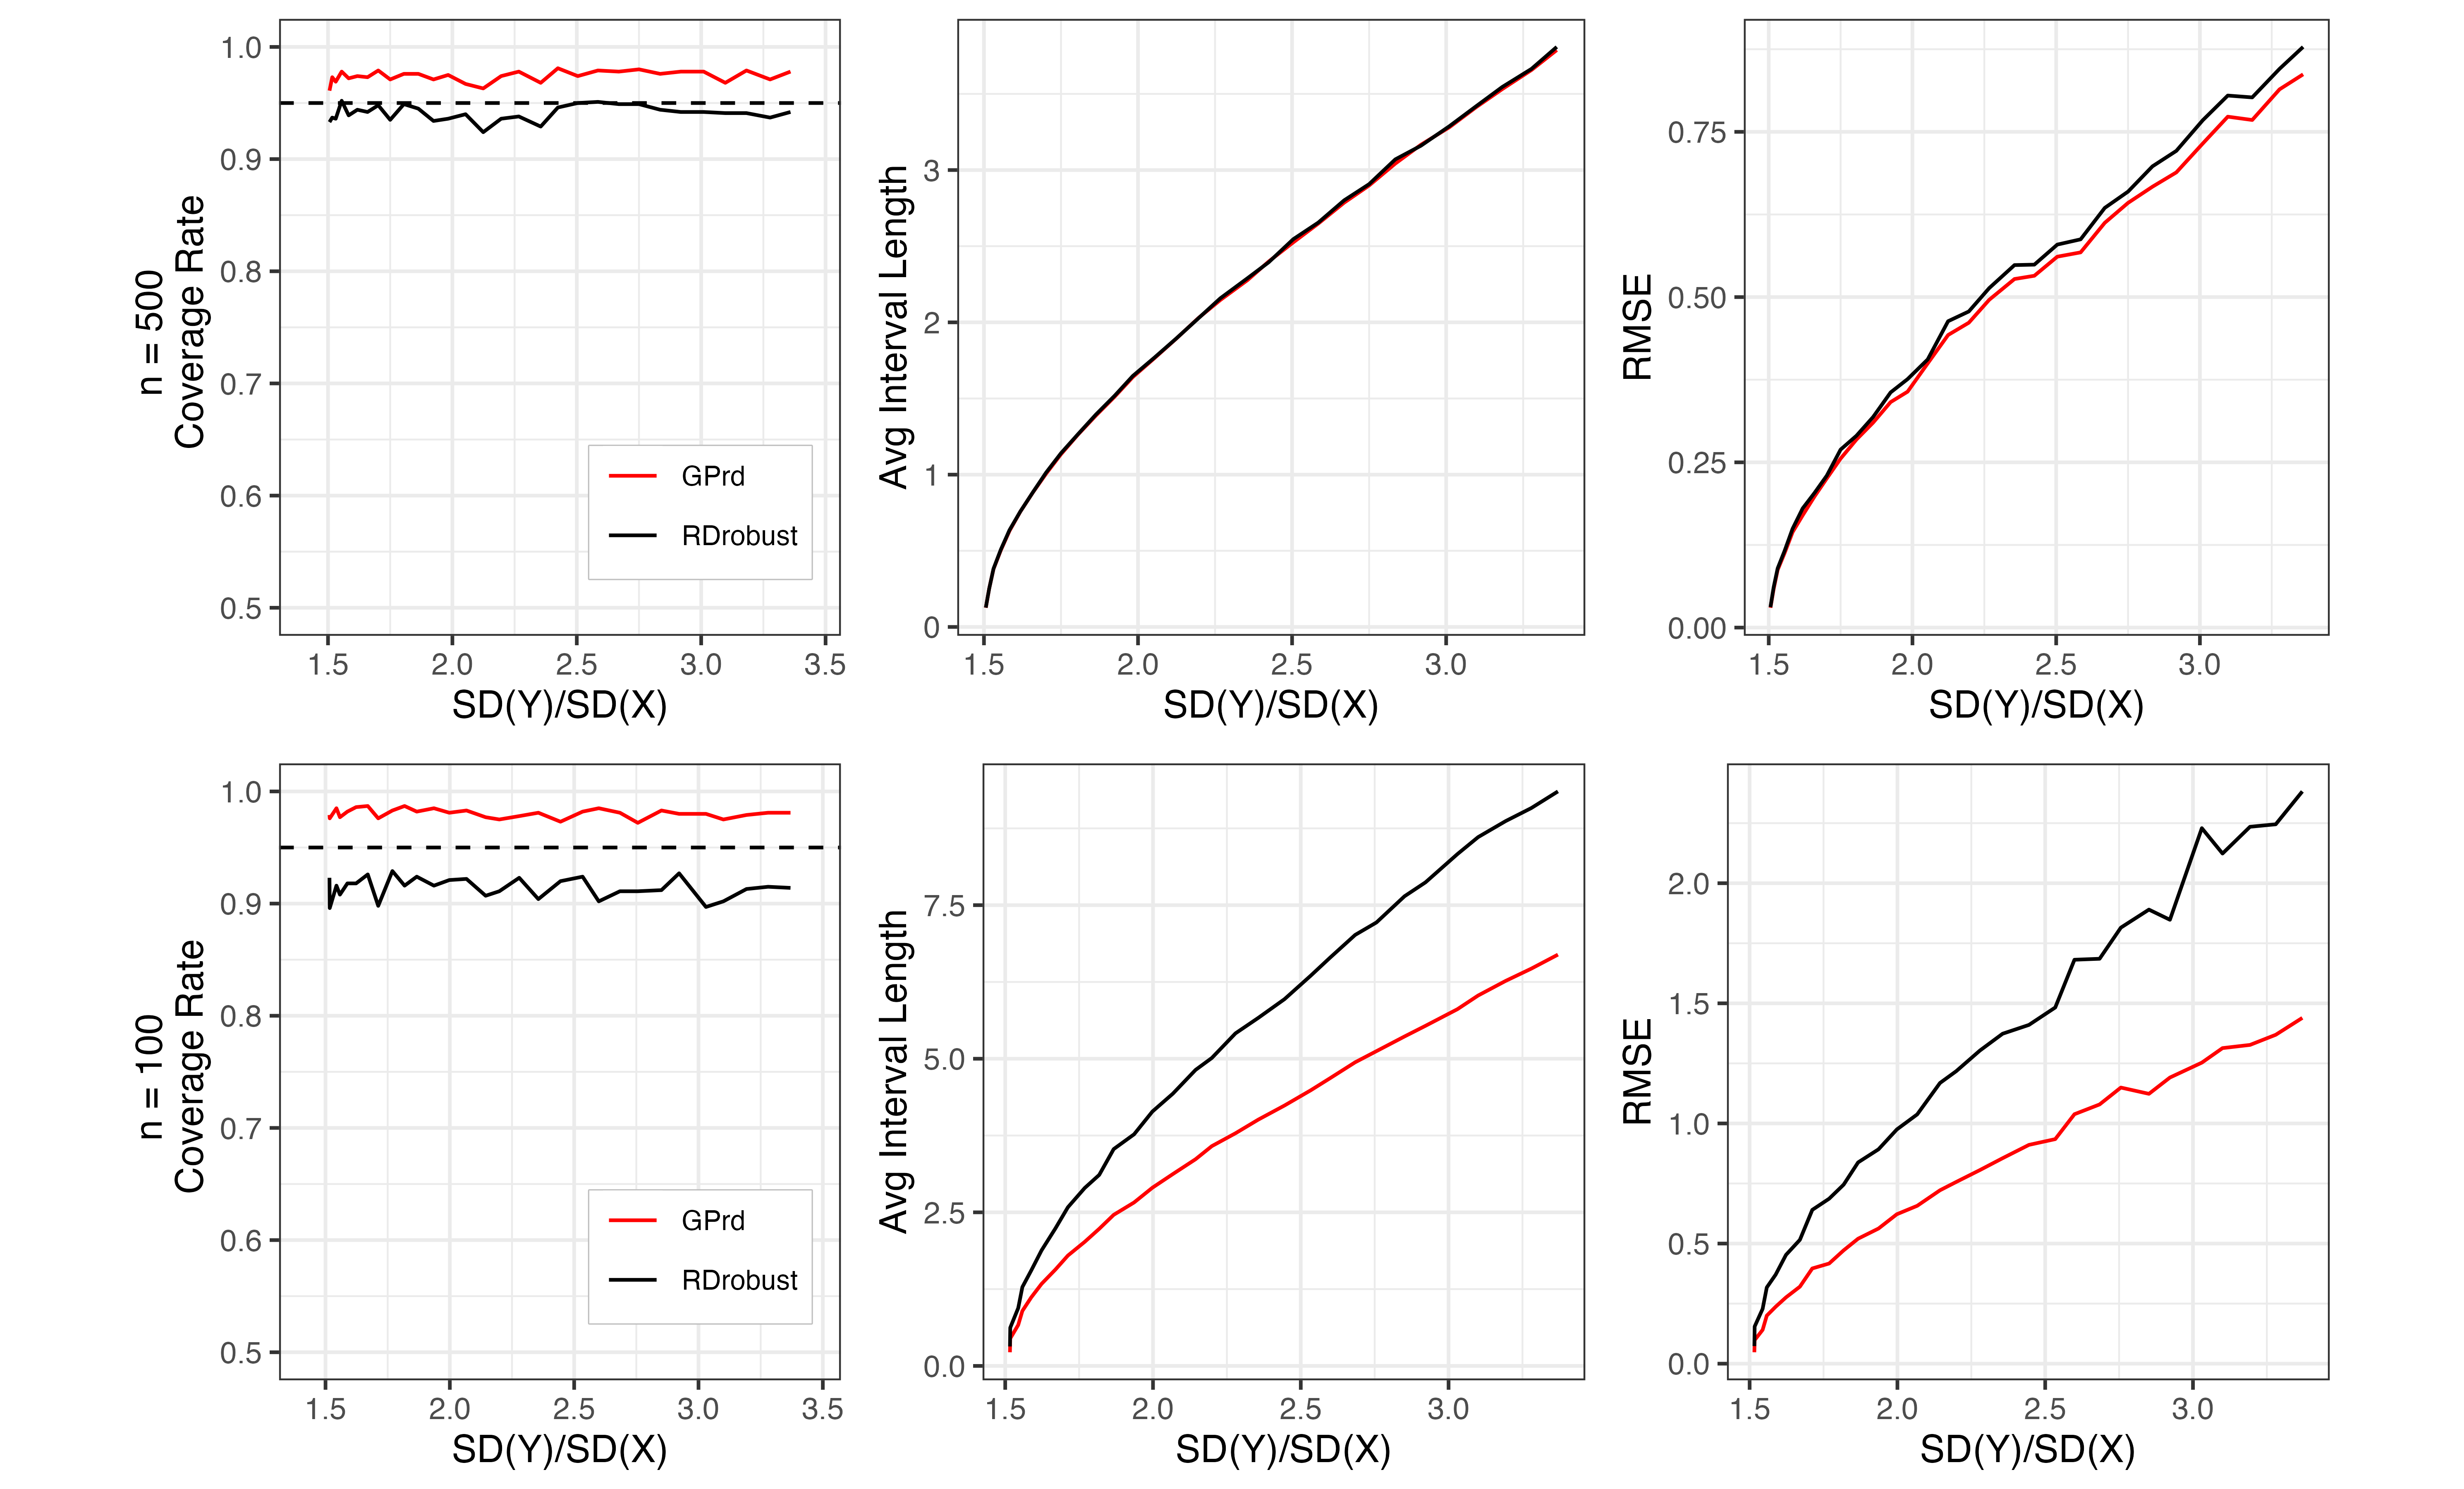
\includegraphics[width=0.8\linewidth]{figures/rdd_totalrandom_tau3_presentation.png}
%     \end{figure}
% \end{frame}

% \begin{frame}{Case 3 RD: simulation with random $Z$ and $Y$ ($\tau = 0$)}
% \begin{center}
%     \begin{figure}[hbt!]
%     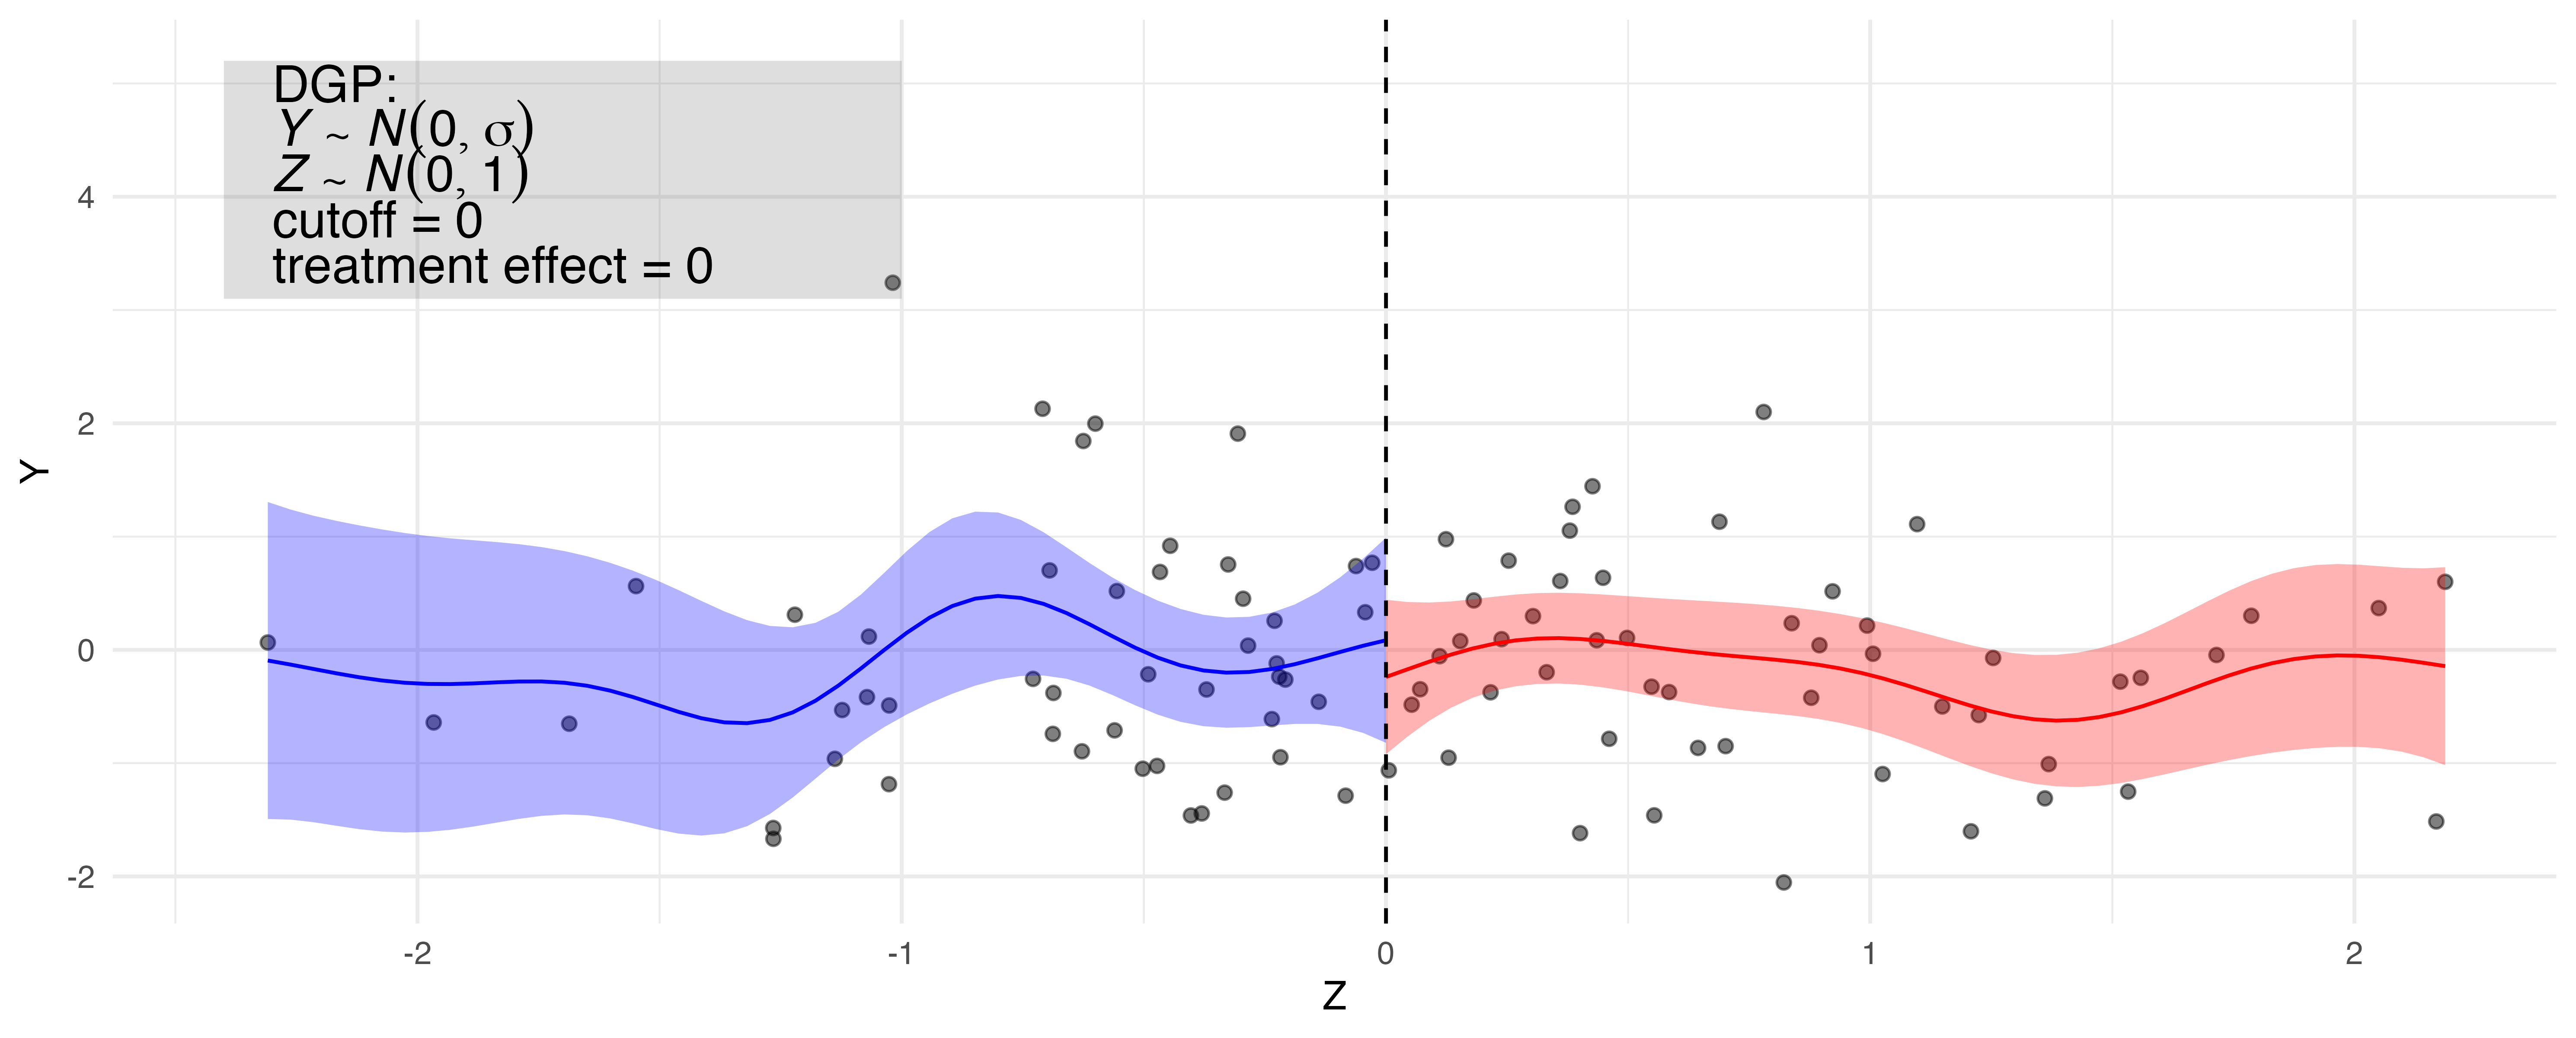
\includegraphics[width=\linewidth]{figures/rdd_sample_tau0.png}
%     \end{figure}
% \end{center}
% \end{frame}

% \begin{frame}{Case 3 RD: simulation with random $Z$ and $Y$ ($\tau = 0$)}
% \vspace{-1.5em}
% \begin{center}
% \end{center}
%     \begin{figure}[hbt!]
%     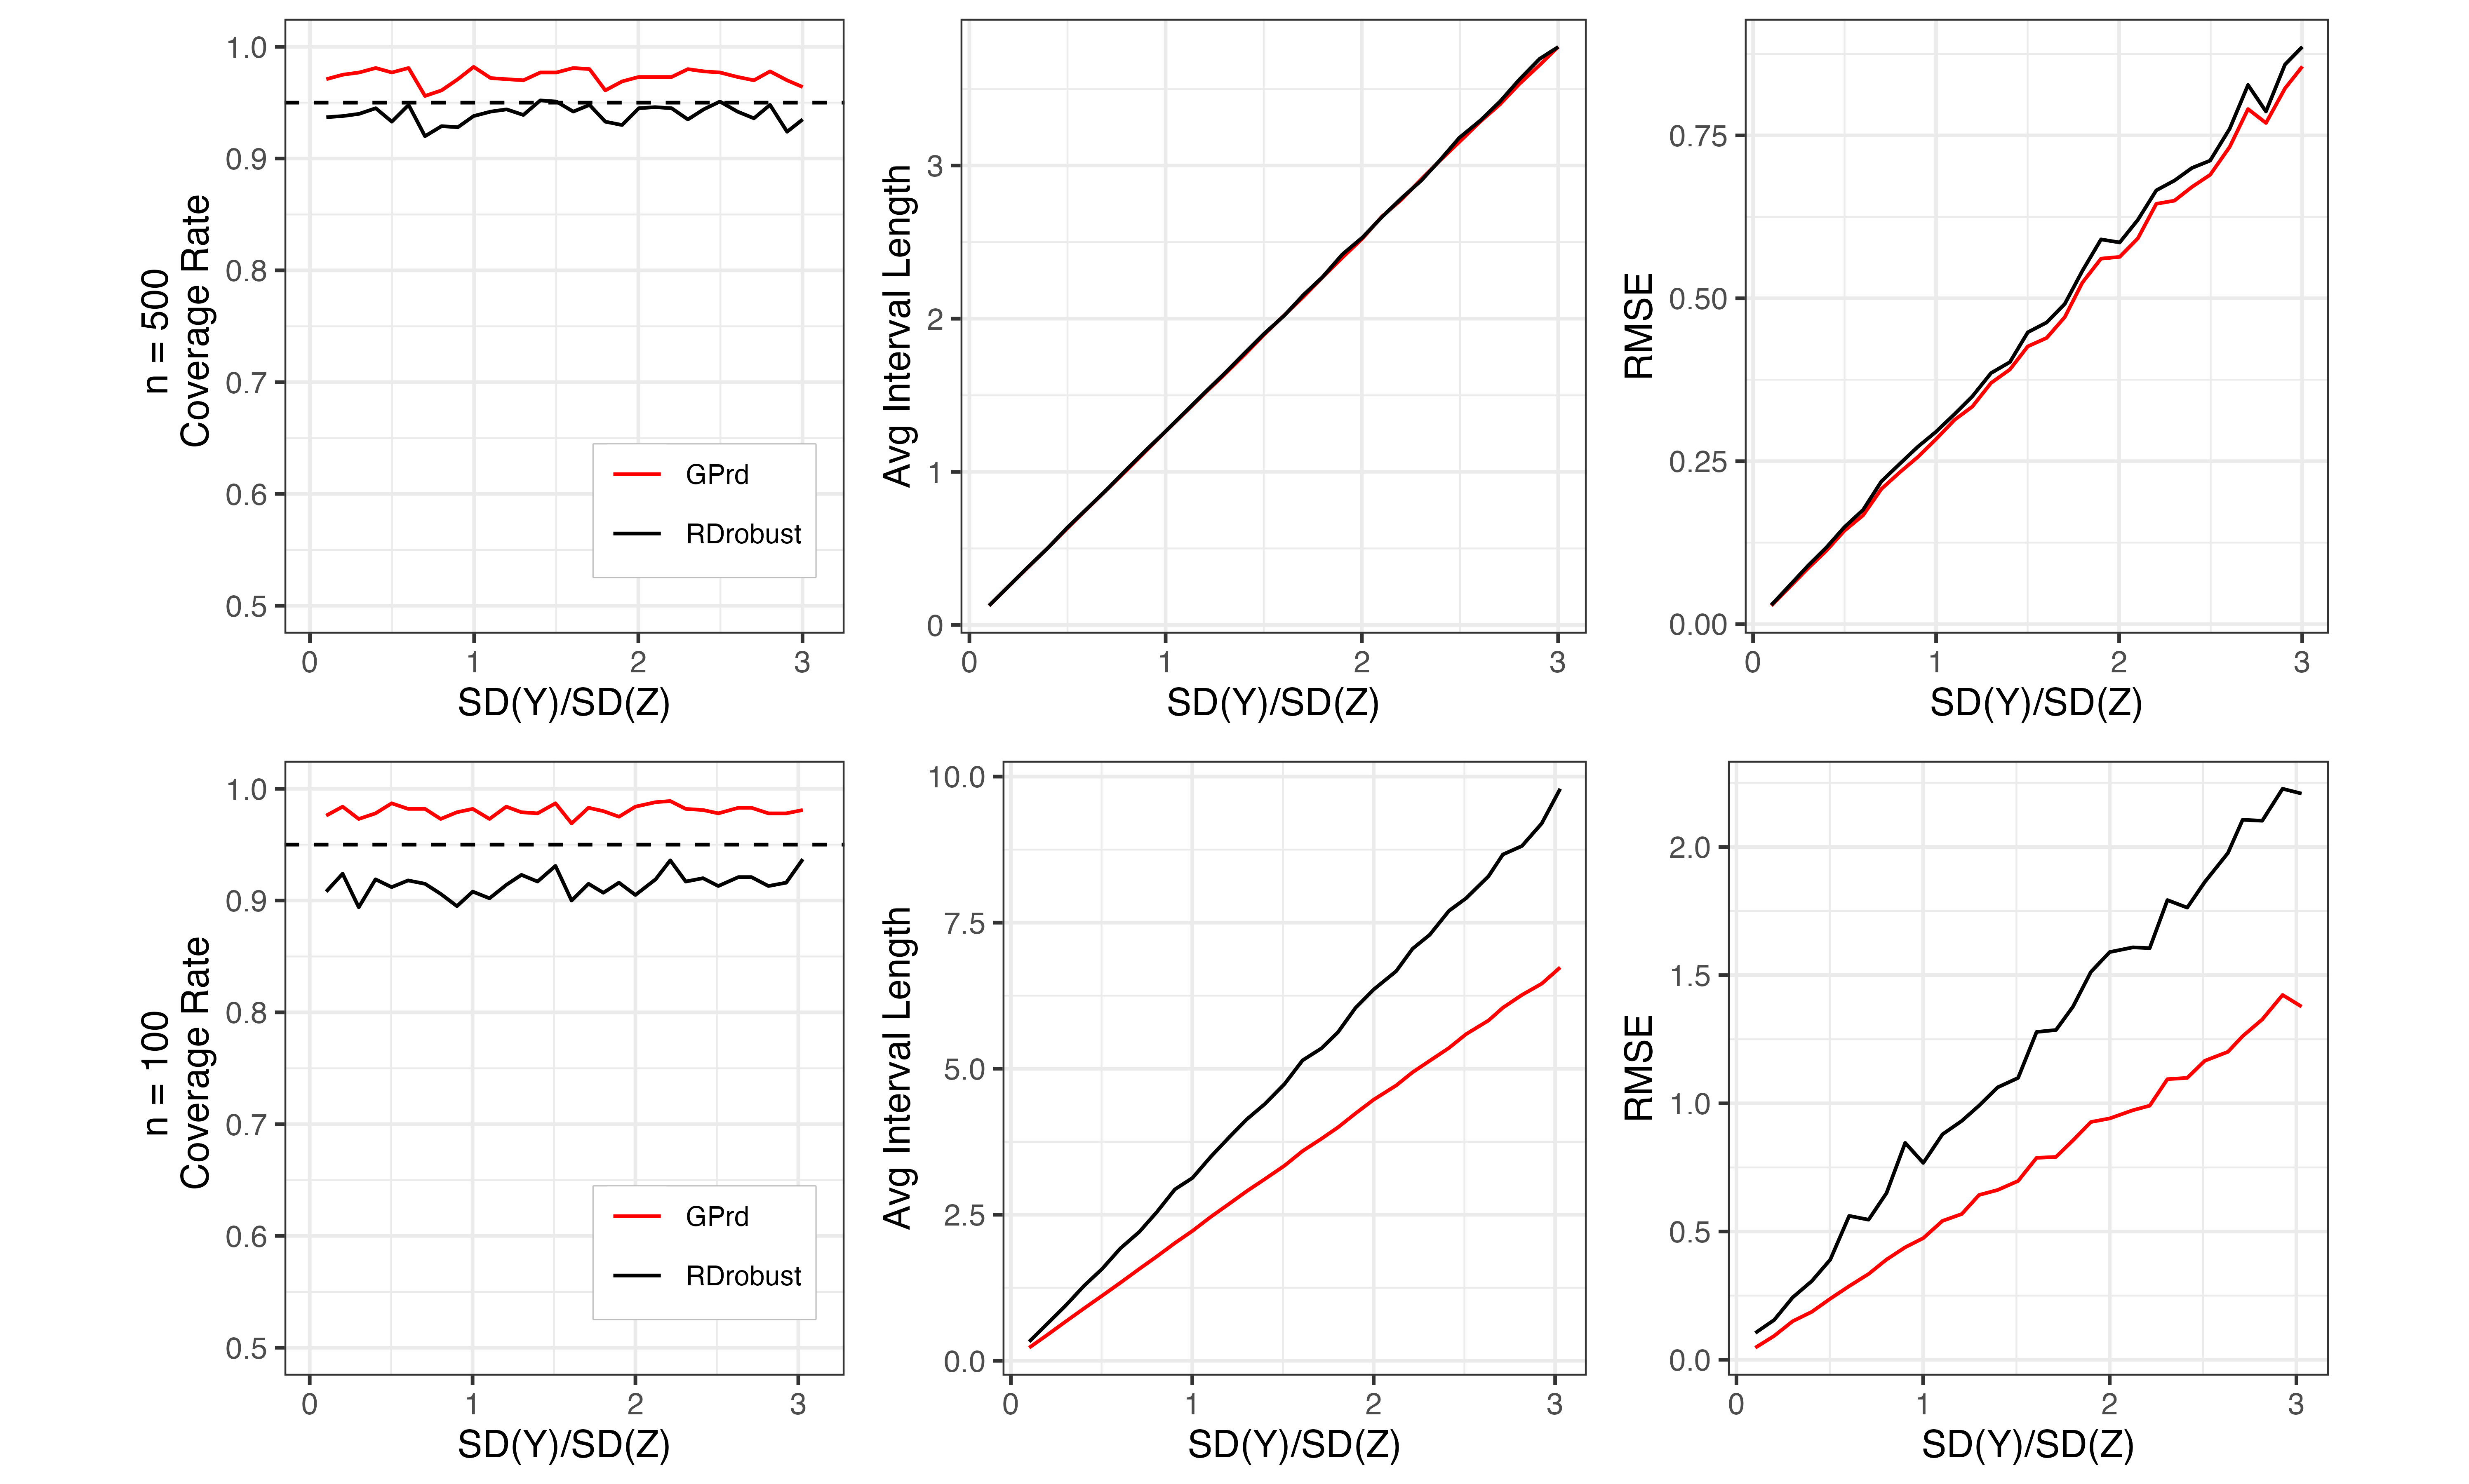
\includegraphics[width=0.8\linewidth]{figures/rdd_totalrandom_tau0_presentation.png}
%     \end{figure}
% \end{frame}

\begin{frame}{Placebo cutoffs in close elections (application)}
Lee (2004) close election setting:
\footnotesize
\begin{itemize}
        \item Forcing variable: Democrats' vote share in US House election (1948 - 1990)
        \item Outcome variable: ADA score (liberal vote score of each representative)
 \end{itemize}
 \bigskip
 \normalsize
 \onslide<2-> Another twist: Should our RD estimates be informed by some \textit{causal assumptions} regarding comparability? 
 \footnotesize
 \begin{itemize}
     \item Should we worry if an automated RD procedure chooses a very wide bandwidth?
     \item In the \texttt{gp\_causaltrim} approach we:
     \begin{enumerate}
     \item use small bandwidth to limit comparison range: e.g. within 2\% vote share, cov=cor=0.9 $\rightarrow$ b=0.005
     \item trim: remove data outside useful range ($\pm 10\%$, so scaling and $\sigma^2$ choice are focused)
%     \item Note: this makes sense under ``local randomization view''; unnecessary in the continuous-PO view?
\end{enumerate}
 \end{itemize}
\end{frame}



\begin{frame}{Placebo cutoffs in close elections: Large sample}
\onslide<1-> \small Full sample: $N=13,577$  (each analysis sees only part of this)
\begin{figure}[hbt!]
\centering
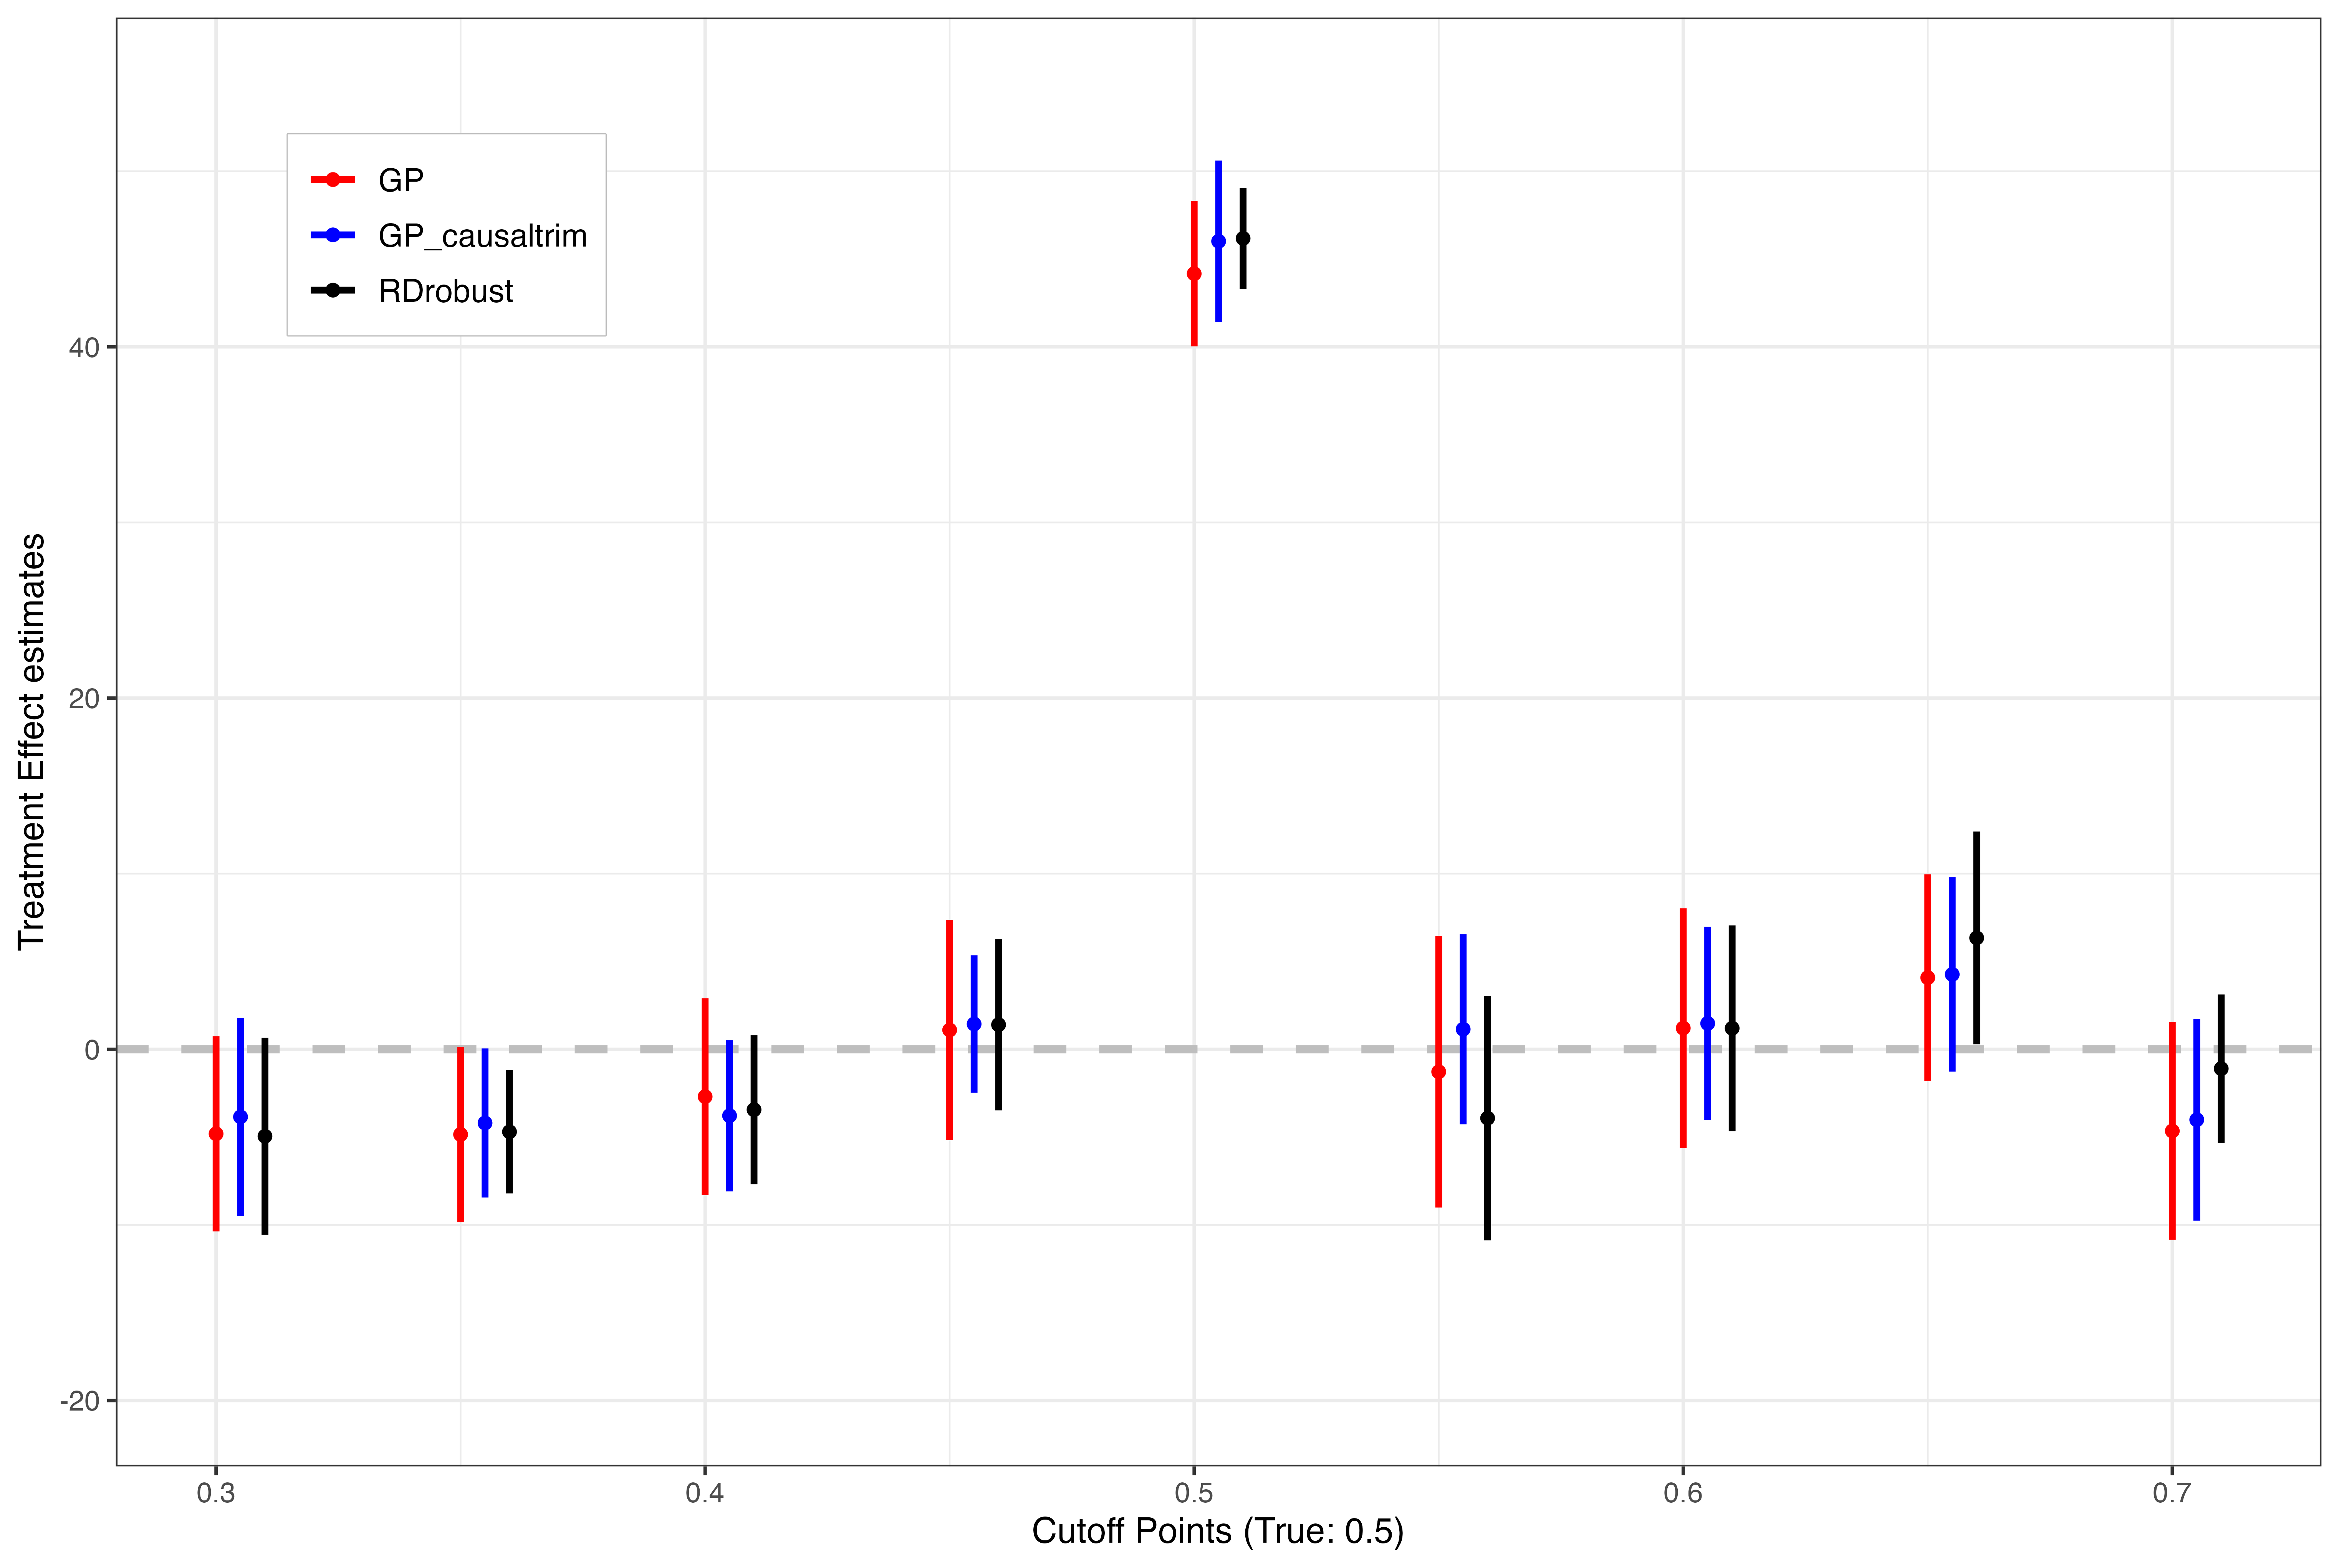
\includegraphics[width=0.6\linewidth]{figures/rdd_Lee_placebo.png}
%\caption{RDD with Close Election Data with Placebo Cutoff Points and Different GP RDD Specifications}
\label{fig:rdd_lee}
\end{figure}
\end{frame}

\begin{frame}{Placebo cutoffs in close elections: Small samples}
\onslide<1-> Repeated sampling of sub-samples: $N=200$ in each segment\\
\begin{figure}[hbt!]
\centering
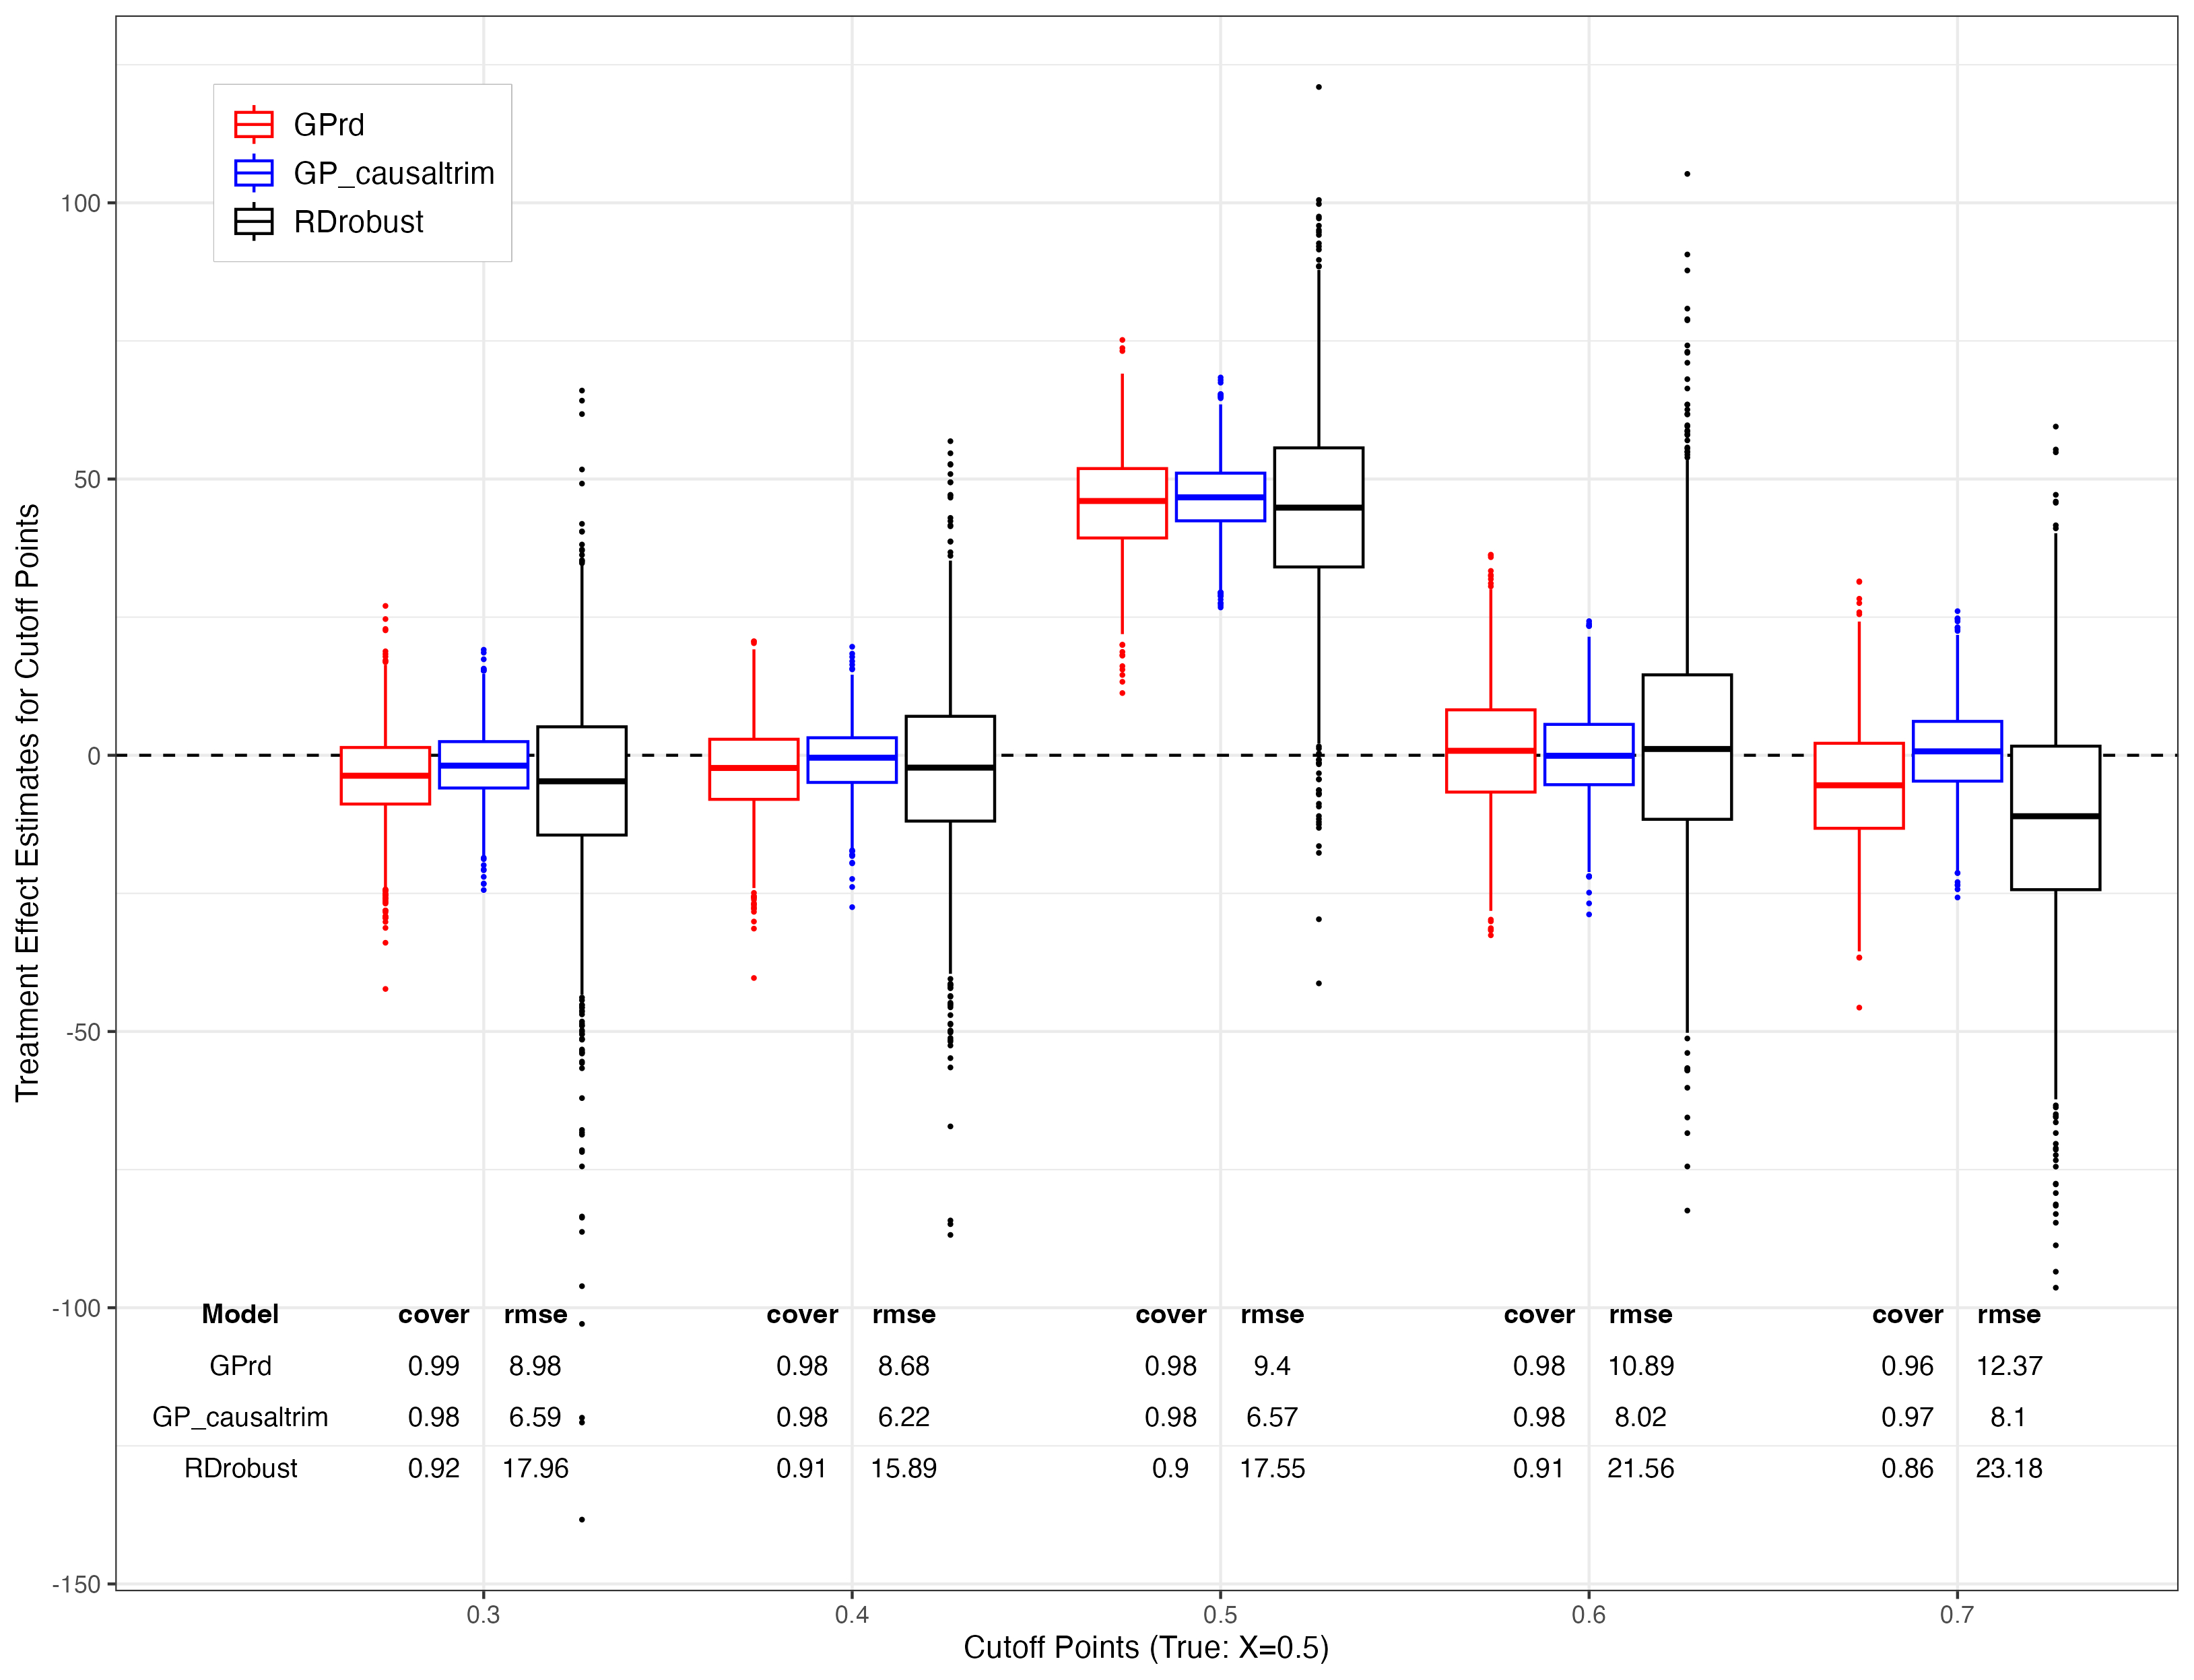
\includegraphics[width=0.65\linewidth]{figures/rdd_Lee_placebo_subsample.png}
\label{fig:rdd_lee}
\end{figure}
%\small
%\onslide<2-> \texttt{GP\_causaltrim}: conveniently does best while being a bit more transparent, restrictive.
\end{frame}

%
%\begin{frame}{Comments on Estimation}
%\onslide<1-> \textcolor{Red}{Practical Advice}
%\small
%\begin{enumerate}
%\item<2-> first, look at scatterplots and run some simple models of your own (e.g. linear or squared with different slopes to left and right. 
%\bigskip
%\item<3-> then use \texttt{rdrobust} or \texttt{RDD} so as  to take bandwidth selection out of your hands
%\bigskip
%\item<4-> you will also need to check for jumps in density of forcing variable and do placebo tests to make sure no covariates jump at threshold (coming soon)
%\end{enumerate}
%
%\end{frame}












%\subsection{Sharp RDD: Estimation}
%
%\begin{frame}
%  \frametitle{Estimating $\alpha_{SRDD}=\E[Y_{1i}|X_i=c]-\E[Y_{0i}|X_i=c]$}
%  \small
%\begin{enumerate}
%\item<1-> Sometimes: start by  trimming sample to small window around the threshold $c$ (discontinuity sample):
%\begin{itemize}
%  \item<2-> For window width $h>0$, use $c-h\leq X_i \leq c + h$, 
%  \item<3-> NB: some estimators are local enough that you don't do this, but you do choose a bandwidth
%\end{itemize}\medskip
%\item<3-> Recode running variable to deviations from threshold: $\tilde{X} = X - c$.
%%\begin{itemize}
%%  \item $\tilde{X} = 0$ if $X=c$
%%  \item $\tilde{X} > 0$ if $X>c$ and thus $D=1$
%%  \item $\tilde{X} < 0$ if $X<c$ and thus $D=0$
%%\end{itemize}\medskip
%\bigskip
%\item<4-> Decide on a model for $\E[Y|X]$ on each side
%\begin{itemize}
%  \item<5-> visual inspection
%  \item<6-> parametric models
%  \item<7-> non/semi-parametric smoothing models
%\end{itemize}
%\end{enumerate}
%\end{frame}
%
%\begin{frame}
%  \frametitle{Sharp RRD Estimation 1: Linear with Same Slope}
%\begin{itemize}
%\item<1-> $\E[Y_{0i}|X]$ is linear and treatment effect, $\alpha$, does not depend on $X_i$:
%\[
%\E[Y_{0i}|X_i]=\mu + \beta X_i \,, \qquad \E[Y_{1i} - Y_{0i} |X_i] =\alpha
%\]
%\item<2-> Therefore $\E[Y_{1i}|X_i] = \alpha + \E[Y_{0i}|X_i] = \alpha + \mu + \beta X_i$
%\item<3-> Since $D_i$ is determined given $X_i$, we have that:
%\begin{eqnarray*}
%  \E[Y_i|X_i,D_i] &=& D\cdot \E[Y_{1i}|X_i] + (1-D_i)\cdot \E[Y_{0i}|X_i] \\
%   &=& \mu + \alpha D_i + \beta X_i \\
%   &=& (\mu + \beta c) + \alpha D_i + \beta (X_i-c) \\
%   &=& \gamma + \alpha D_i + \beta \tilde{X}_i
%\end{eqnarray*}
%\item<4-> So we just run a regression of $Y$ on $D$ and $\tilde{X}$
%\end{itemize}
%\end{frame}
%
%\begin{frame}
%\frametitle{Sharpp RDD: Linear with Same Slope}
%\begin{center} 
%  
\includegraphics[height=3in,keepaspectratio=1]{Re1.pdf}
%  \end{center}
%\end{frame}
%
%%\begin{frame}
%%\frametitle{Sharp RDD: Graphical Illustration Linear Case}
%%  
\includegraphics[height=3.3in,keepaspectratio=1]{rddex2.pdf}
%%\end{frame}
%
%\begin{frame}
%  \frametitle{Sharp RDD Estimation 2: Differential Slopes}
%\begin{itemize}
%\item<1-> Or, let $\E[Y_0|X]$ and $E[Y_1|X]$ be different  linear functions of $X$, so the average effect of the treatment $E[Y_1-Y_0|X]$ varies with $X$:
%\[
%\E[Y_{0i}|X_i]=\mu_0 + \beta_0 X_i, \qquad  E[Y_{1i}|X_i]=\mu_1 + \beta_1 X_i
%\]
%\item<2-> So $\alpha (X)=\E[Y_{1i}-Y_{0i}|X_i]=(\mu_1-\mu_0) + (\beta_1-\beta_0)X_i$ we have
%\begin{align*}
%\E[Y_i|X_i,D_i]=& D_i \cdot \E[Y_{1i}|X_i] + (1-D_i)\cdot \E[Y_{0i}|X_i]\\
%=& \,\,\mu_1 D_i + \beta_1 (X_i \cdot D_i) + \mu_0 (1-D_i) + \beta_0 X_i \cdot (1-D_i)\\
%=& \,\, \gamma + \beta_0 \tilde{X}_i + \alpha D_i + \beta_1 \tilde{X_i}\cdot D_i
%%\end{align*}
%\end{align*}
%\item<3-> Regress $Y_i$ on $\tilde{X}_i$, $D_i$, and the interaction $\tilde{X}_i \cdot D_i$. 
%\item<4-> \textcolor{Blue}{What does each coefficient in the above represent?} %The coefficient of $D$ reflects the average effect of the treatment at $X=c$
%\end{itemize}
%\end{frame}
%
%\begin{frame}
%\frametitle{Sharp RDD: Linear with Differential Slope}
%\begin{center}
%  
\includegraphics[height=3in,keepaspectratio=1]{Re2.pdf}
%  \end{center}
%\end{frame}
%
%\begin{frame}
%  \frametitle{Sharp RDD Estimation 3: More flexible parametric}
%\small
%\onslide<1-> Suppose $\E[Y_0|X]$ and $\E[Y_1|X]$ are separate \textit{non-linear} functions of $X$ and the average effect of the treatment $\E[Y_1-Y_0|X]$ varies with $X$ \\
%\medskip
%\onslide<2-> At minimum, include higher-order terms in $(X-c)$ and their interactions with $D$, e.g.\\
%\begin{align*}
%\E[Y_i|X_i,D_i]=& \gamma_0 + \gamma_1 \tilde{X}_i + \gamma_2 \tilde{X}_i^2\\
%+&\alpha_0 D_i + \alpha_1 (\tilde{X}_i\cdot D_i) + \alpha_2 (\tilde{X}_i^2\cdot D_i)
%\end{align*}
%\onslide<3-> In such cases $\alpha_0 = \E[Y_1-Y_0|X=c]$ estimates effect at $X=c$ \\
%\end{frame}
%
%\begin{frame}
%\frametitle{SRDD: Non-Linear Case}
%\begin{center}
%  
\includegraphics[height=3in,keepaspectratio=1]{Re3.pdf}
%  \end{center}
%\end{frame}
%
%\begin{frame}{Non-parametric estimators}
%\small
%\onslide<1-> In practice we now rely mainly on more local, flexible models such as lowess or kernel smoothers \\
%\medskip
%\onslide<2-> Trimming may not even matter in these, but choice of a ``bandwidth'' does\\
%\medskip
%\onslide<3-> Parametric and non-parametric models are both subject to a bias/variance tradeoff:\\
%\footnotesize
%\begin{itemize}
%\item<4-> more parameters, smaller bandwidth, and narrower trimming all imply more flexibility (lower bias) but greater variability (variance)
%\item<5-> ideal to show results are not sensitive to changes in model, trimming, bandwidth
%\end{itemize}
%\small
%\onslide<6-> Also best to take bandwidth decisions out of your hands:\\
%\footnotesize
%\begin{itemize}
%\item<6-> Imbens-Kalyanaraman (2012): See \texttt{IKbandwidth} in \texttt{RDD} package
%\item<7-> Calonico, Cattaneo, and Titiunik for automatic bandwidth selection for local polynomial models, and automatic algorithms for a range of plots (see \texttt{rdrobust})
%\end{itemize}
%\end{frame}
%
%%\begin{frame}{Comments on Estimation}
%%\onslide<1-> No ex-ante correct model for $\E[Y|X]$ on each side. \\
%%\footnotesize
%%\begin{itemize}
%%\item<2-> bias variance tradeoff: more parameters (or smaller bandwidth) will give more flexible model but depends heavily on small changes in data
%%\item<3-> good practice to show results are not sensitive to changes in model or in the window around $X=c$. 
%%\item<4-> especially important to show you can cut window very narrowly and get similar result (though variance will explode)  
%%\end{itemize}
%%\normalsize
%%\onslide<5-> Automated selection procedures:
%%\footnotesize
%%\begin{itemize}
%%\item<6-> Imbens-Kalyanaraman (2012): See \texttt{IKbandwidth} in \texttt{RDD} package
%%\item<7-> These days: Use Calonico, Cattaneo, and Titiunik for automatic bandwidth selection for local polynomial models, and automatic algorithms for a range of plots \\ (see \texttt{rdrobust})
%%%\item<8-> \textcolor{Red}{Practical advice}: do some simple models (e.g. linear with different slopes) yourself, then use \texttt{rdrobust} and \texttt{RDD} to get reliable estimates.
%%\end{itemize}
%%\end{frame}
%
%
%\begin{frame}{Comments on Estimation}
%\onslide<1-> \textcolor{Red}{Practical Advice}
%\small
%\begin{enumerate}
%\item<2-> first, look at scatterplots and run some simple models of your own (e.g. linear or squared with different slopes to left and right. 
%\bigskip
%\item<3-> then use \texttt{rdrobust} or \texttt{RDD}, to take bandwidth selection out of your hands
%\bigskip
%\item<4-> you also need to do some falsification tests -- next.
%\end{enumerate}
%
%\end{frame}

\subsection{Falsification Checks}

\begin{frame}
\frametitle{Sharp RDD: Falsification Checks}
\small
\begin{enumerate}
\item Specification sensitivity: Are results sensitive to alternative specifications?\bigskip
\item Balance Checks: Do covariates $Z$ jump at the threshold?
\bigskip
\item Check if jumps occur at placebo thresholds $c^{\star}$?
\bigskip
\item Sorting: Do units sort around the threshold? (density test)
\end{enumerate}
\end{frame}

\begin{frame}
\frametitle{Sharp RDD: Risk of Mispecification}
\begin{center}

\includegraphics[scale=.7]{RDDmisspec_1.pdf}
\end{center}
\end{frame}


\begin{frame}
\frametitle{Sharp RDD: Risk of Mispecification}
\begin{center}

\includegraphics[scale=.7]{RDDmisspec_2.pdf}
\end{center}
\end{frame}


\begin{frame}
\frametitle{Sharp RDD: Risk of Mispecification}
\begin{center}
\onslide<1-> Using Imbens-Kalyanaraman bandwidth in \texttt{RDD} \\

\includegraphics[scale=.7]{RDDmisspec_IK.pdf}
\end{center}
\end{frame}

%\begin{frame}
%\frametitle{Sharp RDD: Sensitivity to Specification}
%  
\includegraphics[height=2in,keepaspectratio=1]{ang3.pdf}
%\begin{itemize}
%  \item $Y=f(X)+\alpha D+\varepsilon$: A miss-specified control function $f(X)$ can lead to a spurious jump: Take care not to confuse a nonlinear relation with a discontinuity
%  \item More flexibility (e.g. adding polynomials) reduces bias, decreases efficiency
%  \item Check sensitivity to size of bandwidth (i.e. estimation window)
%\end{itemize}
%\end{frame}

\begin{frame}
\frametitle{SRDD: Balance Test}
\small
\onslide<1-> Test for comparability of agents around the cut-off: \\
\footnotesize
\begin{itemize}
\item<2-> For potential outcomes to be continuous, any  influencer (observed or unobserved) must also be continuous
 %\item<3-> Visual tests: for observed $Z_i$, plot $\E[Z_i|X_i]$ and look for jumps
\item<3-> Consider pre-treatment covariate (or placebo outcome) $Z_i$  
  \item<4-> Run the RDD regression using $Z_i$ as the outcome. Use same estimation as for the real outcome. E.g.,  
  \[ \E[Z_i|X_i,D_i]= \beta_0 + \beta_1 (X_i-c) + \alpha_z D_i + \beta_3 (X_i-c)\cdot D_i \]
should yield $\alpha_z=0$ if $Z$ is balanced at the threshold.
%\begin{itemize}
%  \item If $\alpha_z \neq 0$ this indicates that some other factor $Z$ also changes at the threshold
%\end{itemize}
\end{itemize}\medskip
\small
\onslide<6-> Finding a discontinuity in $Z$ poses a challenge to the identification strategy.\\
\begin{itemize}
\item<7-> if you see imbalance at threshold on a \textcolor{Blue}{post-treatment} variable, is that a problem?
%\item Alternatively, regress the outcome variable on a vector of controls and use the residuals in the RDD, instead of the outcome itself
\end{itemize}\smallskip
\small
\onslide<8-> As usual, balance checks are \textcolor{Red}{falsification} tests. Remember unobservables.
\end{frame}

\begin{frame}
\frametitle{SRDD: Falsification Test}
\begin{center}
  
\includegraphics[height=3in,keepaspectratio=1]{Hidalgo2.pdf}
\end{center}
\end{frame}


%\begin{frame}
%\frametitle{SRDD: You Can Add Covariates}
%\begin{center}
%  
\includegraphics[height=2.6in,keepaspectratio=1]{mp.pdf}
%\end{center}
%\end{frame}


\begin{frame}
\frametitle{SRDD: Falsification Test}
\small
\onslide<1-> Especially convincing to do this with placebo outcome, i.e. covariates likely related to potential outcomes but not influenced by treatment. \\
\vspace{-0in}
\begin{center}
  
\includegraphics[height=2.7in,keepaspectratio=1]{lee2.pdf}
  \end{center}
\end{frame}


%\begin{frame}
%\frametitle{SRDD: Falsification Test}
%\begin{center}
%  
\includegraphics[height=3in,keepaspectratio=1]{egg2.pdf}
%\end{center}
%\end{frame}


\begin{frame}
\frametitle{SRDD: Placebo Thresholds}
\onslide<1-> Let $c^{\star}$ be a placebo threshold value. Run models 
\[ \E[Y_i|X_i,D_i]= \beta_0 + \beta_1 (X_i-c^{\star}) +\alpha_{fake} D_i + \beta_3 (X_i-c^{\star})\cdot D_i \]
\vspace{-.1in} and check if $\alpha_{fake}$ is large and significant.\\
\medskip
\small
\begin{itemize}
  \item<2-> Usually we run separate models below and above $c$, with bandwidth to exclude $c$, to avoid misspecification due to inclusion of the actual jump. 
  \smallskip
\item<3-> Detecting a jump at placebo threshold requires an explanation.
\begin{itemize}
\footnotesize
\item e.g. if other treatments occurred near $c^{\star}$, it could be okay
\item but problematic if it implies unknown treatments or unobserved influences may account for effect at $c$
\item can also reveal specification problems, as your model could be guessing a discontinuous jump occurs where it was actually smooth
\end{itemize}
%\item<5-> Maybe data exists in a period where there was no program
\end{itemize}
\end{frame}

\begin{frame}
\frametitle{SRDD: Sorting}
\onslide<1-> Can subjects \textcolor{Blue}{self-sort} around threshold?
  \begin{itemize}
  \small
    \item<2-> Can they exercise fine control over the running variable?
    \item<3-> Can administrators strategically choose what is used as running variable or as threshold? 
    \item<4-> Either can allow sorting of agents around the cut-off, s.t. those below may differ on average form those just above
        \item<5-> Does not necessarily invalidate the design unless sorting is \textcolor{Blue}{(a)} precise, and \textcolor{Blue}{(b)} widespread
        \begin{itemize}
        \item<6->[(a)] imprecise sorting is okay as long as you can find narrow enough bandwidth around $X=c$ s.t. those to left and right of $c$ are no different
        \item<7->[(b)] if some people can sort very precisely, RDD may be biased but less biased then naive comparison 
        \end{itemize}
  \end{itemize}\bigskip
% \onslide<8-> \textcolor{Blue}{Bundled Treatments}. What else changes at $c$? Bundled treatments can invalidate continuity assumption. 
\end{frame}

\begin{frame}[fragile]
\frametitle{SRDD: Sorting Around the Threshold}
\onslide<1-> Test for discontinuity in density of forcing variable:
\small
  \begin{itemize}
  \item<2-> Visual Histogram Inspection:
  \footnotesize
  \begin{itemize}\medskip
    \item<2-> Construct equal-sized non-overlapping bins of the forcing variable s.t. no bin includes points both above and below $c$ \medskip
    \item<2-> For each bin, compute the number of observations and plot the bins to see if there is a discontinuity at the cut-off
  \end{itemize}\bigskip  
  \small
        \item<3-> Formal test: McCrary (2008)
  \end{itemize}
\end{frame}

\begin{frame}[fragile]
\frametitle{Self-sorting simulation}
\begin{columns}[T] 
     \begin{column}[T]{5cm} 
\scriptsize
\begin{verbatim}
>N=200
>runvar=rnorm(N, mean = 0, sd=1)
>c=.5
>DCdensity(runvar, cutpoint=c)
[1] 0.5857803
\end{verbatim}
\bigskip
\onslide<3->
\begin{verbatim}
> sortprob=rep(0,N)
> sortprob[runvar<c]=.25*exp(runvar[runvar<c]-c)
> selfsorts=rbinom(N, size=1, prob = sortprob)
> runvar[selfsorts==1]=.5+
runif(sum(selfsorts),.001,.5)
> DCdensity(runvar, cutpoint=c)
[1] 0.0001952333
\end{verbatim}
     \end{column}
     \begin{column}{5cm} 
     \footnotesize
\onslide<2-> 
\includegraphics[height=4cm, width=4.5cm]{simulatedMC1.pdf} \\
\onslide<4-> 
\includegraphics[height=4cm, width=4.5cm]{simulatedMC2.pdf} 
     \end{column}
     \end{columns}

\end{frame}

\begin{frame}
\frametitle{Bundled (or just other) Treatments}
\begin{itemize}
\item<1-> The achilles heal of RD identification: other treatments at the same cutoff. 
\bigskip 
\begin{itemize}
\item violates continuity assumpion.
\item essentially a confounder
\end{itemize}
\bigskip
\item<3-> Ask yourself: what else changes at $c$?
\bigskip
\item<4-> Worry about commonly used eligibility criteria, political borders.
\end{itemize}
\end{frame}




%\begin{frame}
%\frametitle{SRDD: Evidence of Sorting}
%Example: Beneficial job training program offered to agents with income $<c$. Concern, people will withhold labor to lower their income below the cut-off to gain access to the program.
%  
\includegraphics[height=1.6in,keepaspectratio=1]{mc1.pdf}
%\end{frame}

%\begin{frame}
%\frametitle{Sorting Around the Threshold (Eggers, 2010)}
%  
\includegraphics[height=2.9in,keepaspectratio=1]{egg6.pdf}
%\end{frame}

%
%
%
%
%\begin{frame}
%\frametitle{SRDD: Sorting Around the Threshold}
%Are units able to manipulate the forcing variable in ways that may be related to the outcomes?
%  
\includegraphics[height=2.5in,keepaspectratio=1]{f1.pdf}
%\end{frame}
%
%
%
%
%
%
%\begin{frame}
%\frametitle{SRDD: Sorting Around the Threshold}
%Is there evidence of manipulation?
%\begin{center}
%  
\includegraphics[height=2.5in,keepaspectratio=1]{Re4.pdf}
%\end{center}
%\end{frame}

\section{Fuzzy Regression Discontinuity Design}

\subsection{Identification}

\begin{frame}
  \frametitle{Fuzzy Regression Discontinuity Design}
\begin{itemize}
\item<1-> Threshold may not perfectly determine treatment
exposure, but it creates a discontinuity in the probability of
treatment exposure\bigskip

\item<2-> Incentives to participate in a program may change discontinuously at a threshold, but the incentives are not powerful enough to move all units from non-participation to participation\bigskip
%\begin{itemize}
%  \item Probability of being offered a scholarship may jump at a certain SAT score (when applicants are given ``special consideration'')
%  \item We shouldn't compare recipients with non-recipients (even close to cut-off) since they are likely differ along
%  unobservables related to outcome (e.g., letters of rec)
%  \item But, we for those applicants with scores close to the cutoff we can exploit the discontinuity as an instrument to estimate the LATE for the subgroup of applicants for whom scholarship receipt depends
%      on position of score relative to cutoff
%      \begin{itemize}
%        \item Compliers are students who switch from non-recipient to recipient if their SAT score cross the cut-off
%      \end{itemize}
%\end{itemize}
%
\item<3-> Should remind you of IV!
\end{itemize}
\onslide<4-> We can use  discontinuities to produce instrumental variable estimators of the effect of the treatment (close to the discontinuity)
\end{frame}

\begin{frame}
  \frametitle{Fuzzy RDD Example:}
\small
\begin{itemize}
  \item<1-> Probability of being offered a scholarship may jump at a certain SAT score threshold (when applicants are given ``special consideration'')\bigskip
  \item<2-> For applicants with scores very close to the threshold:
  \begin{itemize}
  \item<3->  scholarship eligibility should be random (so $Z_i \indep D_{1i}, D_{0i}$)
  \smallskip
  \item<4-> we may think tiny change in score, being nearly random,  only effects outcome through scholarship chances ($Z_i \indep Y_{0i}, Y_{1i}$)
  \smallskip
  \item<5-> If both, we have a good instrument.
  \end{itemize}
  \bigskip
  \item<6-> \textcolor{Blue}{Who are compliers in this framework?} 
\end{itemize}
\end{frame}

%Decision to offer a scholarship based on:
%Continuous measure of academic ability (e.g., GRE) exceeds given cut-off, and
%Subjective information (e.g., recommendation letters) observed only by the evaluator
%Does scholarship receipt impact academic achievement?
%Don’t compare recipients with non-recipients (even close to cut-off) to estimate ATE ? likely differ along unobservables related to outcome (e.g., letters of rec)
%But, could compare average outcomes of all subjects, irrespective of recipient status, just to the left and right of the cut-off…

%The LATE represents the average treatment effect of the compliers
%i.e., the subgroup of individuals whose treatment status would switch from non-recipient to recipient if their score x crossed the cut-off
%The share of this group in the population in the neighborhood of the cut-off is just the denominator of:


\begin{frame}
\frametitle{Fuzzy RDD: Discontinuity in $\E[D|X]$ }
\begin{center}
  
\includegraphics[height=2.9in,keepaspectratio=1]{Fuzzy1.pdf}
\end{center}
\end{frame}

\begin{frame}
\frametitle{Fuzzy RDD: Discontinuity in $\E[Y|X]$ }
\begin{center}
  
\includegraphics[height=2.9in,keepaspectratio=1]{R22.pdf}
\end{center}
\end{frame}

\begin{frame}
  \frametitle{Fuzzy RDD: Identification}
%\onslide<1-> Binary instrument $Z$ with $Z=\mathbbm{1}_{\{X>c\}}$\\ 
%\onslide<2-> Restrict estimation/sample to observations close to discontinuity, $X \approx c$
\onslide<1-> \begin{iass}
\footnotesize
For sufficiently small $\epsilon$ s.t. $X_i-\epsilon<c<X_i+\epsilon$, we have usual IV assumption:
\begin{enumerate}
\item<2-> Ignorability (and Exclusion):  $\{Y_{1i},Y_{0i},D_{1i},D_{0i} \} \indep Z_i $
\item<3-> Relevance: $\E[D_{1i}] \neq \E[D_{0i}]$
\item<4-> Monotoniticy: $D_{1i} \geq D_{0i} \; \forall i$
\end{enumerate}
\end{iass}
\onslide<5->
\begin{ires}
\footnotesize
\begin{align*}
 \alpha_{FRDD}  &= \E[Y_{1i}-Y_{0i} | X_i=c \mbox{ and }\, \,i\,\, \mbox{ is a complier} ] \\
  &=   \frac{\lim_{x\downarrow c}\E[Y_i|X_i=c]-\lim_{x\uparrow c}\E[Y_i|X_i=c]}{\lim_{x\downarrow c}\E[D_i|X_i=c]-\lim_{x\uparrow c}\E[D_i|X_i=c]} \\
  &= \frac{\mbox{outcome discontinuity}}{\mbox{treatment discontinuity}} \\
  &\approx \frac{\hat{\E}[Y|Z=1, X=c]-\hat{\E}[Y|Z=0, X=c]}{\hat{\E}[D|Z=1, X=c]-\hat{\E}[D|Z=0, X=c]}
\end{align*}
\end{ires}
\end{frame}

%\begin{frame}
%\frametitle{Fuzzy RDD: Identification}
%\begin{itemize}
%\item Suppose $E[Y_0|X]$ is linear and treatment effect is constant:
%\[
%E[Y_0|X] = \mu + \beta X, \,\, E[Y_1-Y_0|X]=\alpha,\,\, E[Y_1|X] = \alpha + \mu + \beta X.
%\]
%\item Suppose also that $E[D|X]$ has a discontinuity at $c$. For those who
%are close to $c$, the average outcomes are:
%\begin{eqnarray*}
%E[Y|Z=0] &=& \mu + \alpha E[D|Z=0] + \beta E[X|Z=0]\\
%E[Y|Z=1] &=& \mu + \alpha E[D|Z=1] + \beta E[X|Z=1]
%\end{eqnarray*}
%\item For those with $X \approx c$ $E[X|Z=1] - E[X|Z=0] \approx 0$. However,
%$E[D|Z=1]-E[D|Z=0]\neq0$ because of discontinuity in the assignment probability
%\end{itemize}
%\end{frame}

\subsection{Estimation}

\begin{frame}
  \frametitle{Fuzzy RDD: Estimation}
  \small
  \begin{itemize}
  \item<1-> Cut the sample to a small window above and below the threshold (discontinuity sample)
  \smallskip
      \item<2-> Code instrument $Z_i=\mathbbm{1}_{\{X>c\}}$
      \smallskip
      \item<3-> Fit 2SLS/IV: $Y_i=\beta_0+\beta_1 (X_i-c) + \beta_2 Z_i (X_i-c) + \alpha D_i$\\
      where $D_i$ is instrumented with $Z_i$
      \smallskip
      \item<4-> Better: use polynomials 
  %    \item Using a larger window we may also fit 2SLS: $Y=\beta_0 + \beta_1 (X-c) + \alpha D + \beta_2 (D*(X-c))$\\
  %    where $D$ and $D*(X-c)$ are instrumented with $Z$ and $Z\cdot(X-c)$
      \item<5-> Better still:  estimate the outcome discontinuity and treatment discontinuity, then divide. Can use any estimator this way. \texttt{rdrobust} can do this for you.  
  \end{itemize}
\end{frame}

\subsection{Fuzzy RDD Example: Early Release from Prison}

\begin{frame}
  \frametitle{Early Release Program (HDC)}
  \begin{itemize}
  \item<1-> Prison system in many countries is faced with overcrowding and high recidivism rates after release.
  \item<2-> Early discharge of prisoners with electronic monitoring has become a popular policy
  \item<3-> Difficult to estimate impact of early release program on future criminal behaviour: best behaved inmates are usually the ones to be released early.
  \item<4-> Marie (2008) considers Home Detention Curfew (HDC) scheme in England and Wales:
  \begin{itemize}
    \item<5-> Fuzzy RDD: Only offenders sentenced to more than 88 days in prison are eligible for HDC, but obviously, not all those with longer sentences are offered HDC
  \end{itemize}
  \item<6-> \textcolor{Blue}{How valid are the identification assumptions?} 
  \end{itemize}
\end{frame}

\begin{frame}
%\frametitle{Fuzzy RDD: Discontinuity in $E[Y|X]$ }
\begin{center}
  
\includegraphics[height=2.9in,keepaspectratio=1]{fuz1.pdf}
\end{center}
\end{frame}

\begin{frame}
%\frametitle{Fuzzy RDD: Discontinuity in $E[Y|X]$ }
\begin{center}
  
\includegraphics[height=2.9in,keepaspectratio=1]{fuz2.pdf}
\end{center}
\end{frame}

\begin{frame}
%\frametitle{Fuzzy RDD: Discontinuity in $E[Y|X]$ }
\begin{center}
  
\includegraphics[height=2.9in,keepaspectratio=1]{fuz3.pdf}
\end{center}
\end{frame}

\begin{frame}
%\frametitle{Fuzzy RDD: Discontinuity in $E[Y|X]$ }
\begin{center}
  
\includegraphics[height=2.9in,keepaspectratio=1]{fuz4.pdf}
\end{center}
\end{frame}

\begin{frame}
%\frametitle{Fuzzy RDD: Discontinuity in $E[Y|X]$ }
\begin{center}
  
\includegraphics[height=2.7in,keepaspectratio=1]{fuz6.pdf}
\end{center}
\begin{center}
\onslide<2-> \textcolor{Blue}{For what group is this the ATE?}
\end{center}
\end{frame}

%\section{RDD Further Issues}

\begin{frame}
  \frametitle{Internal and External Validity}
  \small
  \onslide<1-> Internal validity:\\
  \footnotesize
  \begin{itemize}
  \item Because the continuity of POs is sometimes reasonably defensible, RDD tends to be more credible
  \item Even if imperfect it is likely to be bias reducing
  \item Main threats tend to be other treatments at same threshold, and specification problems.
  \end{itemize}
  \small
  \onslide<2-> External validity:\\
  \begin{itemize}
  \footnotesize
  	\item<3-> You get the average effect of the sub-population with $X_i$ close to $c$
	\item<3-> Fuzzy RDD further restricts this to the compliers with $X_i$ close to $c$
	\item<3-> Only with strong assumptions (e.g., homogenous treatment effects) can we estimate the overall average treatment effect
	 \end{itemize}
\end{frame}

%\section{Are Close Elections Random?}
%
%\begin{frame}
%  \frametitle{Imbalance in lagged incumbency, U.S.\ House 1946-2010}
%\begin{figure}[h]
%%\caption*{Figure A3:}
%\centering
%
\includegraphics[scale=0.8]{fig1_alt.pdf}
%\end{figure}
%\end{frame}
%
%\begin{frame}
%  \frametitle{p-values for ``effect'' of winning$_t$ on winning$_{t-1}$ }
%  \scriptsize
%\begin{center}\setlength{\baselineskip}{10pt}
%\begin{tabular}{|l|c|c|c|c|c|c|c|}
%\hline
%%& \multicolumn{2}{|c|}{}      & \multicolumn{3}{|c|}{}             & \multicolumn{2}{|c|}{}           \\ %[-.10in]
%& \multicolumn{2}{|c}{Naive} & \multicolumn{3}{c|}{Local Linear} & \multicolumn{2}{c|}{Polynomial} \\ %[.05in]
%\hline
%%& & & & & & & \\
%\multicolumn{1}{|r|}{{\it Bandwidth} $=$} &~ {\it .5} ~&~ {\it 1} ~&~ {\it 1} ~&~ {\it 2} ~&~ {\it 5} ~&~ {\it 5} ~&~ {\it 10} \\ %[.05in]
%\hline
%%& & & & & & & \\ [-.10in]
%U.S., House of Reps, 1880-2010  & {\rm .11} & {\rm .06} & {\rm .46} & {\rm .29} & {\rm .32} & {\rm .29} & {\rm .32} \\% [.03in]
%~~ U.S., House of Reps, 1880-1944  & {\it .70} & {\rm .96} & {\it .59} & {\it .38} & {\it .93} & {\it .50} & {\it .65} \\ %[.03in]
%~~ U.S., House of Reps, 1946-2010  & \alert{{\rm .00}} & \alert{{\rm .00}} & \alert{{\rm .04}} & \alert{{\rm .00}} & {\rm .07} & \alert{{\rm .00}} & \alert{{\rm .02}} \\ %[.03in]
%U.S., Statewide, 1946-2010  & {\it .55} & {\it .79} & {\it .43} & {\it .38} & {\it .56} & {\it .50} & {\it .10} \\ %[.03in]
%U.S., State Legislature, 1990-2010  & {\it .37} & {\rm .52} & {\it .32} & {\rm .95} & {\rm .59} & {\it .78} & {\it .77} \\ %[.03in]
%U.S., Mayors, 1947-2007  & --  & {\rm .96} & --  & {\rm .81} & {\rm .88} & {\rm .37} & {\it .62} \\ %[.03in]
%\pause
%Canada, Commons, 1867-2011  & {\it .29} & {\it .50} & {\it .32} & {\it .18} & {\it .09} & {\it .59} & {\it .17} \\ %[.03in]
%~~ Canada, Commons, 1867-1911  & {\it .59} & {\it .22} & {\rm .81} & {\it .21} & {\it .19} & {\it .60} & {\it .18} \\ %[.03in]
%~~ Canada, Commons, 1921-2011  & {\it .30} & {\it .88} & {\it .18} & {\it .39} & {\it .17} & {\it .71} & {\it .35} \\ %[.03in]
%U.K., Commons, 1918-2010  & {\rm .33} & {\rm .09} & {\rm .59} & {\rm .61} & {\rm .08} & {\it .92} & {\rm .12} \\ %[.03in]
%U.K., Local Councils, 1946-2010  & {\rm .24} & {\rm .06} & {\rm .44} & {\rm .27} & {\rm .22} & {\rm .17} & {\rm .68} \\ %[.03in]
%Germany, Bundestag, 1953-2009  & {\rm .71} & {\rm .54} & {\rm .79} & {\rm .48} & {\it 1.00} & {\rm .74} & {\rm .84} \\ %[.03in]
%Bavaria, Mayors, 1948-2009  & {\it .13} & {\it .38} & {\it .21} & {\it .39} & {\it .16} & {\it .19} & {\it .30} \\ %[.03in]
%France, Natl Assembly, 1958-2007  & {\rm .27} & {\rm .79} & {\rm .33} & {\rm .55} & {\rm .53} & {\rm .47} & {\rm .23} \\ %[.03in]
%France, Municipalities, 2008  & --  & {\rm .31} & --  & {\rm .37} & {\rm .14} & {\rm .52} & {\rm .24} \\ %[.03in]
%Australia, House of Reps, 1987-2007  & --  & --  & --  & {\rm 1.00} & {\it .55} & {\rm .50} & {\it .92} \\ %[.03in]
%New Zealand, Parliament, 1949-1987  & --  & --  & --  & --  & {\rm .75} & {\it .86} & {\rm .69} \\ %[.03in]
%India, Lower House, 1977-2004  & {\rm .49} & {\rm .38} & {\it .54} & {\it .98} & {\rm .20} & {\it .97} & {\rm .86} \\ %[.03in]
%Brazil, Mayors, 2000-2008  & {\it .81} & {\it .81} & {\it .61} & {\it .58} & {\rm .78} & {\it .64} & {\rm .97} \\ %[.03in]
%Mexico, Mayors, 1970-2009  & {\it .69} & {\it .96} & {\it .39} & {\it .68} & {\it .93} & {\it .93} & {\it .60} \\ %[.03in]
%\hline
%%& & & & & & & \\ [-.10in]
%All Races Pooled  & {\rm .22} & \alert{{\rm .02}} & {\rm .92} & {\rm .59} & {\rm .16} & {\rm .46} & {\rm .75} \\ %[.03in]
%\hline
%\end{tabular}
%\end{center}
%\end{frame}
%
%\begin{frame}
%\frametitle{t-values for ``effect'' of winning$_t$ on winning$_{t-1}$}
%\begin{figure}[tbp]
%\centering
%
\includegraphics[scale=0.6]{t_stat_histograms_lagged_victory.pdf}
%\end{figure}
%\end{frame}
%
%
%\begin{frame}
%  \frametitle{Testing for imbalances in lagged incumbent victory}
%\begin{figure}[h]
%%\caption*{Figure A3:}
%\centering
%
\includegraphics[scale=.8, trim=0 0 0 0]{lag_victory_graph_pooled}
%\end{figure}
%\end{frame}
%
%\begin{frame}
%  \frametitle{Testing for imbalances in lagged incumbent victory}
%\begin{figure}[h]
%%\caption*{Figure A3:}
%\centering
%
\includegraphics[scale=.8, trim=30 0 0 0]{lag_victory_graphs}
%\end{figure}
%\end{frame}
%
%\begin{frame}
% \frametitle{Conclusion}
%  \small
%\begin{enumerate}
%  \item Eggers et al (2014) results suggest that recent concerns about validity of electoral RD designs are overblown
%\begin{itemize}
%  \item across more than 40,000 close races in many different settings, they find no systematic evidence of sorting
% % \item absence of convincing theory to explain post-war House imbalance suggests it might be a statistical fluke
%\end{itemize} 
% \item Does do not excuse researchers that use electoral RD designs from support their identifying assumptions with evidence
% \begin{itemize}
%   \item placebo effects of the treatment on the lagged outcome, running, and treatment variable, and other pre-treatment covariates along with tests for sorting based on McCrary
%  % \item Check robustness across specifications 
%   \item advantage of RD design is that it lends itself to these numerous tests
%   \item reverting back to traditional regression is not the solution!
% \end{itemize}
% \item Extra care is required for RD analysis in post-war U.S.\ House: 
%\end{enumerate}
%\end{frame}

%\begin{frame}
%  \frametitle{Multiple Thresholds: Effect of Class Size}
%  \begin{itemize}
%\item Old Jewish law (Mainomides) says class size should not be over 40.  Angrist and Lavy (1999)
%look at schools where cohorts are close to multiples of 40.
%\item If just over a multiple, the actual class size is much smaller than if the cohort size is just under 40.
%\item Within that set of classes they look at correlation between educational outcomes test score and class size.
%\end{itemize}
%\end{frame}
%
%\begin{frame}
%\frametitle{Class Size Effect}
%\vspace{-.2in}
%\begin{center}
%  
\includegraphics[height=2.6in,keepaspectratio=1]{ang1.pdf}
%\end{center}
%\end{frame}
%
%\begin{frame}
%\frametitle{Class Size Effect}
%\vspace{-.2in}
%\begin{center}
%  
\includegraphics[height=2.6in,keepaspectratio=1]{ang2.pdf}
%\end{center}
%\end{frame}

%\begin{frame}
%\frametitle{Sharp RDD Example: Effect of Reading Program}
%
%\begin{itemize}
%\item Evaluation of a compensatory reading program
%conducted among second-graders in Providence (RI) in the late 70's
%\item Comprehensive Test of Basic Skill was administered to students in 1978. Those who scored below
%certain cutoff were assigned to a compensatory reading program
%\item $Y$: a second test administered to the same students in 1979
%\item $X$: is the pre-test score
%\item $D$ is assignment to the compensatory reading program
%\item The compensatory reading program is
%estimated to increase CTBS scores by 45 points
%\end{itemize}
%\end{frame}
%
%\begin{frame}
%\frametitle{Sharp RDD Example: Effect of Reading Program}
%  
\includegraphics[height=3.2in,keepaspectratio=1]{rddex5.pdf}
%\end{frame}
%
%\begin{frame}
%\frametitle{Sharp RDD Example: Effect of Reading Program}
%  
\includegraphics[height=2.7in,keepaspectratio=1]{rddex6.pdf}
%\end{frame}
%
%\begin{frame}
%\frametitle{Sharp RDD Example: Effect of Reading Program}
%  
\includegraphics[height=2.7in,keepaspectratio=1]{rddex7.pdf}
%\end{frame}
%
%


\end{document}
